
\newpage
\section{Introduction}

% TODO: Flash criticised for accessibility issues (c.f. Google Docs canvas rendering)
% (similar in aiming for more control / deep embedding) - cf. Ankerson book
% (also HotWired banner ads before popus?) - see onenote
%
% TODO: c.f. Aureli - economic city (urbus) took over political city (civita)
% dtto with open source taking over free software
% (tldr https://chatgpt.com/c/68ae3b00-ccd0-8333-a4ac-f66d14725ab0)
% ~
%
Most software that is built today is a black box. What the users of the software can do is
determined by the software design and the decisions of its designers and programmers remain hidden in
the program source code. In most cases, users do not have access to the source code.\endnote{A typical
situation with online services and apps including, for example, social networks and AI chatbots.}
Even when the source code is available,\endnote{In case of open-source software such
as the Linux operating system, the Firefox web browser or the LibreOffice office suite.} its complexity
and structure makes it practically impossible for most users to answer questions about the inner
workings of the software.

The black box nature of software has wide-ranging consequences. It means that end-users have no
way of finding out why they are seeing particular results when using the software and how those results
were obtained. For example, they cannot find out why they are seeing a specific advertisement on
social media and they have no way of adapting software to suit their accessibility needs.
There are numerous attempts to address those limitations. Work on \emph{explainable AI}\endnote{See for
example review by \citet{dwivedi-2023-xai}.} aims to make artificial intelligence models more
transparent, \emph{enabling architecture}\endnote{\citet{clark-2014-gpii} imagines Global Public Inclusive
Infrastructure that enables personal digital inclusion.} supports building of inclusive
adaptable applications and \emph{malleable software}\endnote{Abstractly characterised by
\citet{tchernavskij-2019-malleable} and illustrated for example by Wildcard \citep{litt-2020-enduser}.}
empowers end-users to modify their software. Despite the virtuous aims of these
approaches, they are treating merely the symptoms of a more basic
limitation of our present way of engaging with software.

Our relationship with software resembles the troublesome relationship of the
society with technical objects that has been studied by Gilbert Simondon in the
1950s.\endnote{His thesis \emph{On the Mode of Existence of Technical Objects} was published
in French in 1958, but the first official English translation only appeared in 2017
\citep{simondon-2017-existence}.} Simondon examined the sources of alienation,
arguing that the ``most powerful cause of alienation in the contemporary world
resides in this misunderstanding of the machine, (...) by the non-knowledge of its
nature and its essence.''\endnote{\citet[p.16]{simondon-2017-existence}}
Today, when software is increasingly ingrained in a wide range of aspects of our lives,
and our ``non-knowledge of its nature and its essence'' is ubiquitous,
the ``most powerful cause of alienation in the contemporary world'' may well be the
misunderstanding of software. At a time when the society needs to make important decisions
about software, the opacity of software prevents us from developing an effective conceptual framework for
understanding how software operates. The fact that most software is intentionally built to hide
its inner workings is a crucial part of that. As Simondon pointed out already, the ``technical
objects that produce the greatest alienation are those meant for ignorant
users.''\endnote{\citet[p.255]{simondon-2017-existence}}

The opaque nature of software is not a necessity. The history of programming offers
many visions of a more open software. The Free Software movement envisioned software
that gives users the freedom to ``study how [it] works and adapt it to [their]
needs,''\endnote{This particular wording is from the ``What is Free Software?'' page
published on the GNU website in 1997 \citep{fsf-1997-free}, but similar ideas already appear
in the first bulletin of the Free Software Foundation \citep{stallman-1986-fsf}.}
while the creators of the Smalltalk programming language in the 1970s saw their system as
``a general purpose meta-medium that anyone can adapt to their particular
needs.''\endnote{Quoted from \citet{kay-1977-media}. The language itself has been
described by \citet{goldberg-1983-smalltalk}. See also historical reflections
by \citet{kay-1993-earlyhistory}.} Such software could empower users
to engage more closely with software and, possibly, also help develop a better understanding
of software in the broader society. Yet, despite these appealing visions, often backed by
solid engineering developments, opaque software remains the~norm.

Understanding how software becomes opaque is the necessary prerequisite for
undoing the closing of software. As argued by Federica Frabetti, if we want to tackle the
deep opacity\endnote{\citet{frabetti-2014-theory} adopts the term used
by \citet{stiegler-1998-technics} who maintains that ``we do not immediately understand what
is being played out in technics (...) even though we unceasingly have to make decisions regarding
technics the consequences of which are felt to escape us more and more.''}
of software, we need ``to problemaitize the intertwining of the technical and the social aspects of
software''\endnote{\citet[p.xix]{frabetti-2014-theory}} and question ``the conceptual system
on which [software] relies for its functioning.''\endnote{\citet[p.xiii]{frabetti-2014-theory}}
Frabetti does this by critically interrogating ``historical-cultural and technical narratives,''
including the origins of software engineering and reflections on free and open software.
I follow a more historical approach. Taking inspiration from the methodology of critical
software studies,\endnote{The book edited by \citet{fuller-2008-lexicon} introduces the field;
specific approaches include critical code studies \citep{marino-2020-critical}, studies of
singular artifacts such as a BASIC one-liner interrogated by \citet{montfort-2012-10print}
or rethinking of the history and origins of software \citep{sack-2019-arts}.}
I closely examine two specific historical case studies (\S\ref{sec:info} and \S\ref{sec:web})
and use them to document how decisions regarding software opacity are made. Before doing so,
I review notable past visions of open software~(\S\ref{sec:visions}) and classify the
different notions of software openness that appear in this article (\S\ref{sec:openness}).

\section{Visions of open software}
\label{sec:visions}

Multiple past visions of software included openness as their key component.
Many of those visions had a profound impact on the computing industry, but in a
remarkable number of cases, the idea of a more open software later got lost.\endnote{This
review is inevitably incomplete. Many more systems would deserve a mention,
including Boxer \citep{disessa-1986-boxer}, Lisp Machines, Interlisp \citep{steele-1996-lisp}
and Emacs \citep{stallaman-1981-emacs}.}

\subsection{Smalltalk}
The Smalltalk programming language was envisioned as the software side of the Dynabook,
a ``personal dynamic medium the size of a notebook which [could] handle
virtually all of its owner's information-related needs.''\endnote{\citet{kay-1977-media}} The language
was intended as ``a general purpose meta-medium that anyone can adapt to their particular
needs.'' This means that a ``kid may turn [the Dynabook] into a painting system, a musician may turn it
into an audio synthesis system and a decision theorist can turn it into an agent-based simulation
system.''\endnote{\citet{petricek-2025-cultures}}

Openness was a necessary part of the vision, because it enabled users understand how the system
works and learn how to modify it:\endnote{This idea was illustrated in an article presenting Smalltalk
in the 1981 issue of the BYTE magazine \citep{reenskaug-1981-user}.}

\begin{quote}
The new user of a Smalltalk system is likely to begin by using its ready-made application
systems for writing and illustrating documents, for designing aircraft wings, for doing homework,
for searching through old court decisions, for composing music, or whatever.

After a while, he
may become curious as to how his system works. He should then be able to ``open up'' the
application object on the screen to see its component parts and to find out how they work~together.

The next thing the user might want to do is to build new systems similar to the one he has been
using. A kit of graphical building blocks would let the user compose a new system (...).
Finally, the expert user would want to make his own kits.
\end{quote}

Today, Smalltalk is recognized as the first object-oriented programming language.
Object-oriented languages like Java adopted many of the Smalltalk language features,
but not the openness of the medium. If you have a running Java
application, you cannot ``open it up'' to find out how it works and adapt
it.\endnote{Although the iPad has the form-factor of the Dynabook that Alan Kay envisioned in
the 1970s, Kay criticised its closed nature arguing that iPad ``could not be farther from the
original intention''~\citep{greelish-2013-kay}.}

The development through which the open object-orientation of Smalltalk turned into
the closed object-orientation of Java has been described as the shift from the humanistic to the
engineering culture of programming.\endnote{\cite{petricek-2025-cultures}} While the former emphasized
openness as a value, the latter was concerned with practical engineering issues such as
deployment, which was challenging in the original Smalltalk~model.\endnote{The issues with
deployment have been listed as one of the possible reasons
for the demise of Smalltalk~\citep{bracha-2020-bits}.}

\subsection{Microcomputers}
In the 1970s, Smalltalk required an expensive special-purpose hardware that was
only available at Xerox PARC. What made computers more widely accessible
was a parallel development.\endnote{This common narrative has been questioned by \citet{rankin-2018-computing},
who points out that access to microcomputers was still limited to an elite group and that
there were other computer networks based on time-sharing systems at the same time.}
Microcomputers were a new kind of computers enabled by the development of
microprocessors.\endnote{Advertised as ``computer on a chip''.} At first, microcomputers were
toys for highly technical tinkerers, but they soon became more powerful and user-friendly.

The ``1977 trinity,''\endnote{The term ``1977 trinity'' only appeared in later written
retrospectives. A detailed account of the history of microcomputers has been written by
\citet{haigh-2021-newhistory}.} comprising Commodore PET, Apple II and TRS-80 sold millions of units.
The way these microcomputers worked was
remarkably close to Alan Kay's vision.\endnote{\citet{petricek-2025-cultures}}
The machines booted into an
interactive BASIC programming prompt and even playing a game involved typing program
commands. The code of BASIC programs was accessible to modification and was often copied
line-by-line from magazines, exposing regular computer users to programming.\endnote{Inspired by
the complementary science methodology \citep{chang-2004-temperature}, the web-based
Commodore 64 BASIC reconstruction (\url{https://tomasp.net/commodore64}) documents interesting
ways of working of the system that have been lost.}

The early open spirit of microcomputers did not last. Developers started
creating more sophisticated applications for microcomputers and many of those were not coded in
BASIC, but in low-level and more opaque assembly. This was frequently for performance reasons.
Many microcomputer users also stopped thinking about them as general-purpose programmable systems, but
as devices to run a specific application. As documented by Laine
Nooney,\endnote{\citet{nooney-2023-appleage}} the Wall Street users referred to Apple II
as the ``VisiCalc machine,'' using the name of an early spreadsheet application, their primary
reason for buying the computer.

\subsection{Free software}
A more ideological approach to the openness of software in the Research Laboratory of Electronics
(RLE) at MIT in the 1960s. The computer programmers who congregated around the TX-0 and PDP-1
computers developed a set of values that were later referred to as the hacker
culture.\endnote{The term was popularized by \citet{raymond-1999-revenge} and
\citet{levy-1984-hackers}. A more critical reflection has recently been written by
\citet{tozzi-2017-fun}.} Hackers believed that access to computers and information should be
unlimited. Anyone should be able to look at program source code, learn from it and modify it
for their own use.

The values were made more explicit when the Free Software Foundation was established in 1985,
possibly in response to the slow demise of the original community of hackers at MIT.
The foundation was ``dedicated to eliminating restrictions on copying, redistribution,
understanding and modification of software.''\endnote{According to the first bulletin published
by the foundation \citep{stallman-1986-fsf}.} The word ``free'' in the name of the organization
referred to two essential freedoms that the foundation aimed to promote, ``the freedom to copy
a program and redistribute it'' and ``the freedom to change a
program.''\endnote{\citet{stallman-1986-fsf}} The latter freedom also required that the source
code of the program is available to its users. To support the aim, the foundation later created
the GPL license, which formalized the requirement. GPL-licensed software must be distributed
with source code and anyone who modifies and redistributes it must also share the modified
source code.

In principle, sharing the source code provides the user with full access to all information
they need to understand how the program works. For the kind of software tools developed as part
of the GNU project in the 1980s, the access to source code also allowed their users to ``change
the program'' in practice. However, this was partly because the users were themselves programmers
and partly because the complexity of the software tools was limited. The degree to which
access to source code enables users to ``change a program'' today may be questioned.
Open source systems like Linux or Firefox are distributed with
source code, yet making even a small change to the software, such as changing the text of
a menu item, is outside of the reach of a vast majority of their users.

\subsection{Hypertext and the Web}
Another software lineage with its own vision of openness is centered around what later became
known as hypertext. The development can be traced to a 1945 essay \emph{As We May Think} by
Vannevar Bush.\endnote{\citet{bush-1945-memex}} In the essay, Bush describes a device for managing
information that makes it possible to follow connections between different documents it
stores.\endnote{Writing in 1945, Bush imagined the documents would be stored on microfilms.}
Bush's essay was influential and later inspired Ted Nelson, who introduced the term `hypertext'.
For our discussion about software openness, it is useful to focus on two later instances of the
idea, the HyperCard application and the World Wide Web.

HyperCard was built by Bill Atkinson for Apple in 1987. Unlike Smalltalk or GNU, which were
programming systems, HyperCard was an end-user application. Users could create ``stacks of
cards'' that contained user interface elements and data. The cards could be linked, so that
clicking a button led the viewer to another card and more complex logic could be implemented
using scripts. HyperCard had an
enthusiastic community of users who used it for a wide range of personal, creative and bussiness
projects. Arguably, one of the reasons for its success was its openness. HyperCard made no strict
distinction between the stack creator and viewer. Both viewing and editing was done in the
same graphical user interface. To edit a stack, the user merely had to switch to a different user
level (Figure~\ref{fig:hypercard}), which added additional controls for modifying the
cards.\endnote{For commercial distribution, it was also possible to lock and password-protect
HyperCard stacks to disable editing, but many stacks were available unlocked and unprotected.}

\begin{figure}
\centering
\vspace{-0.5em}
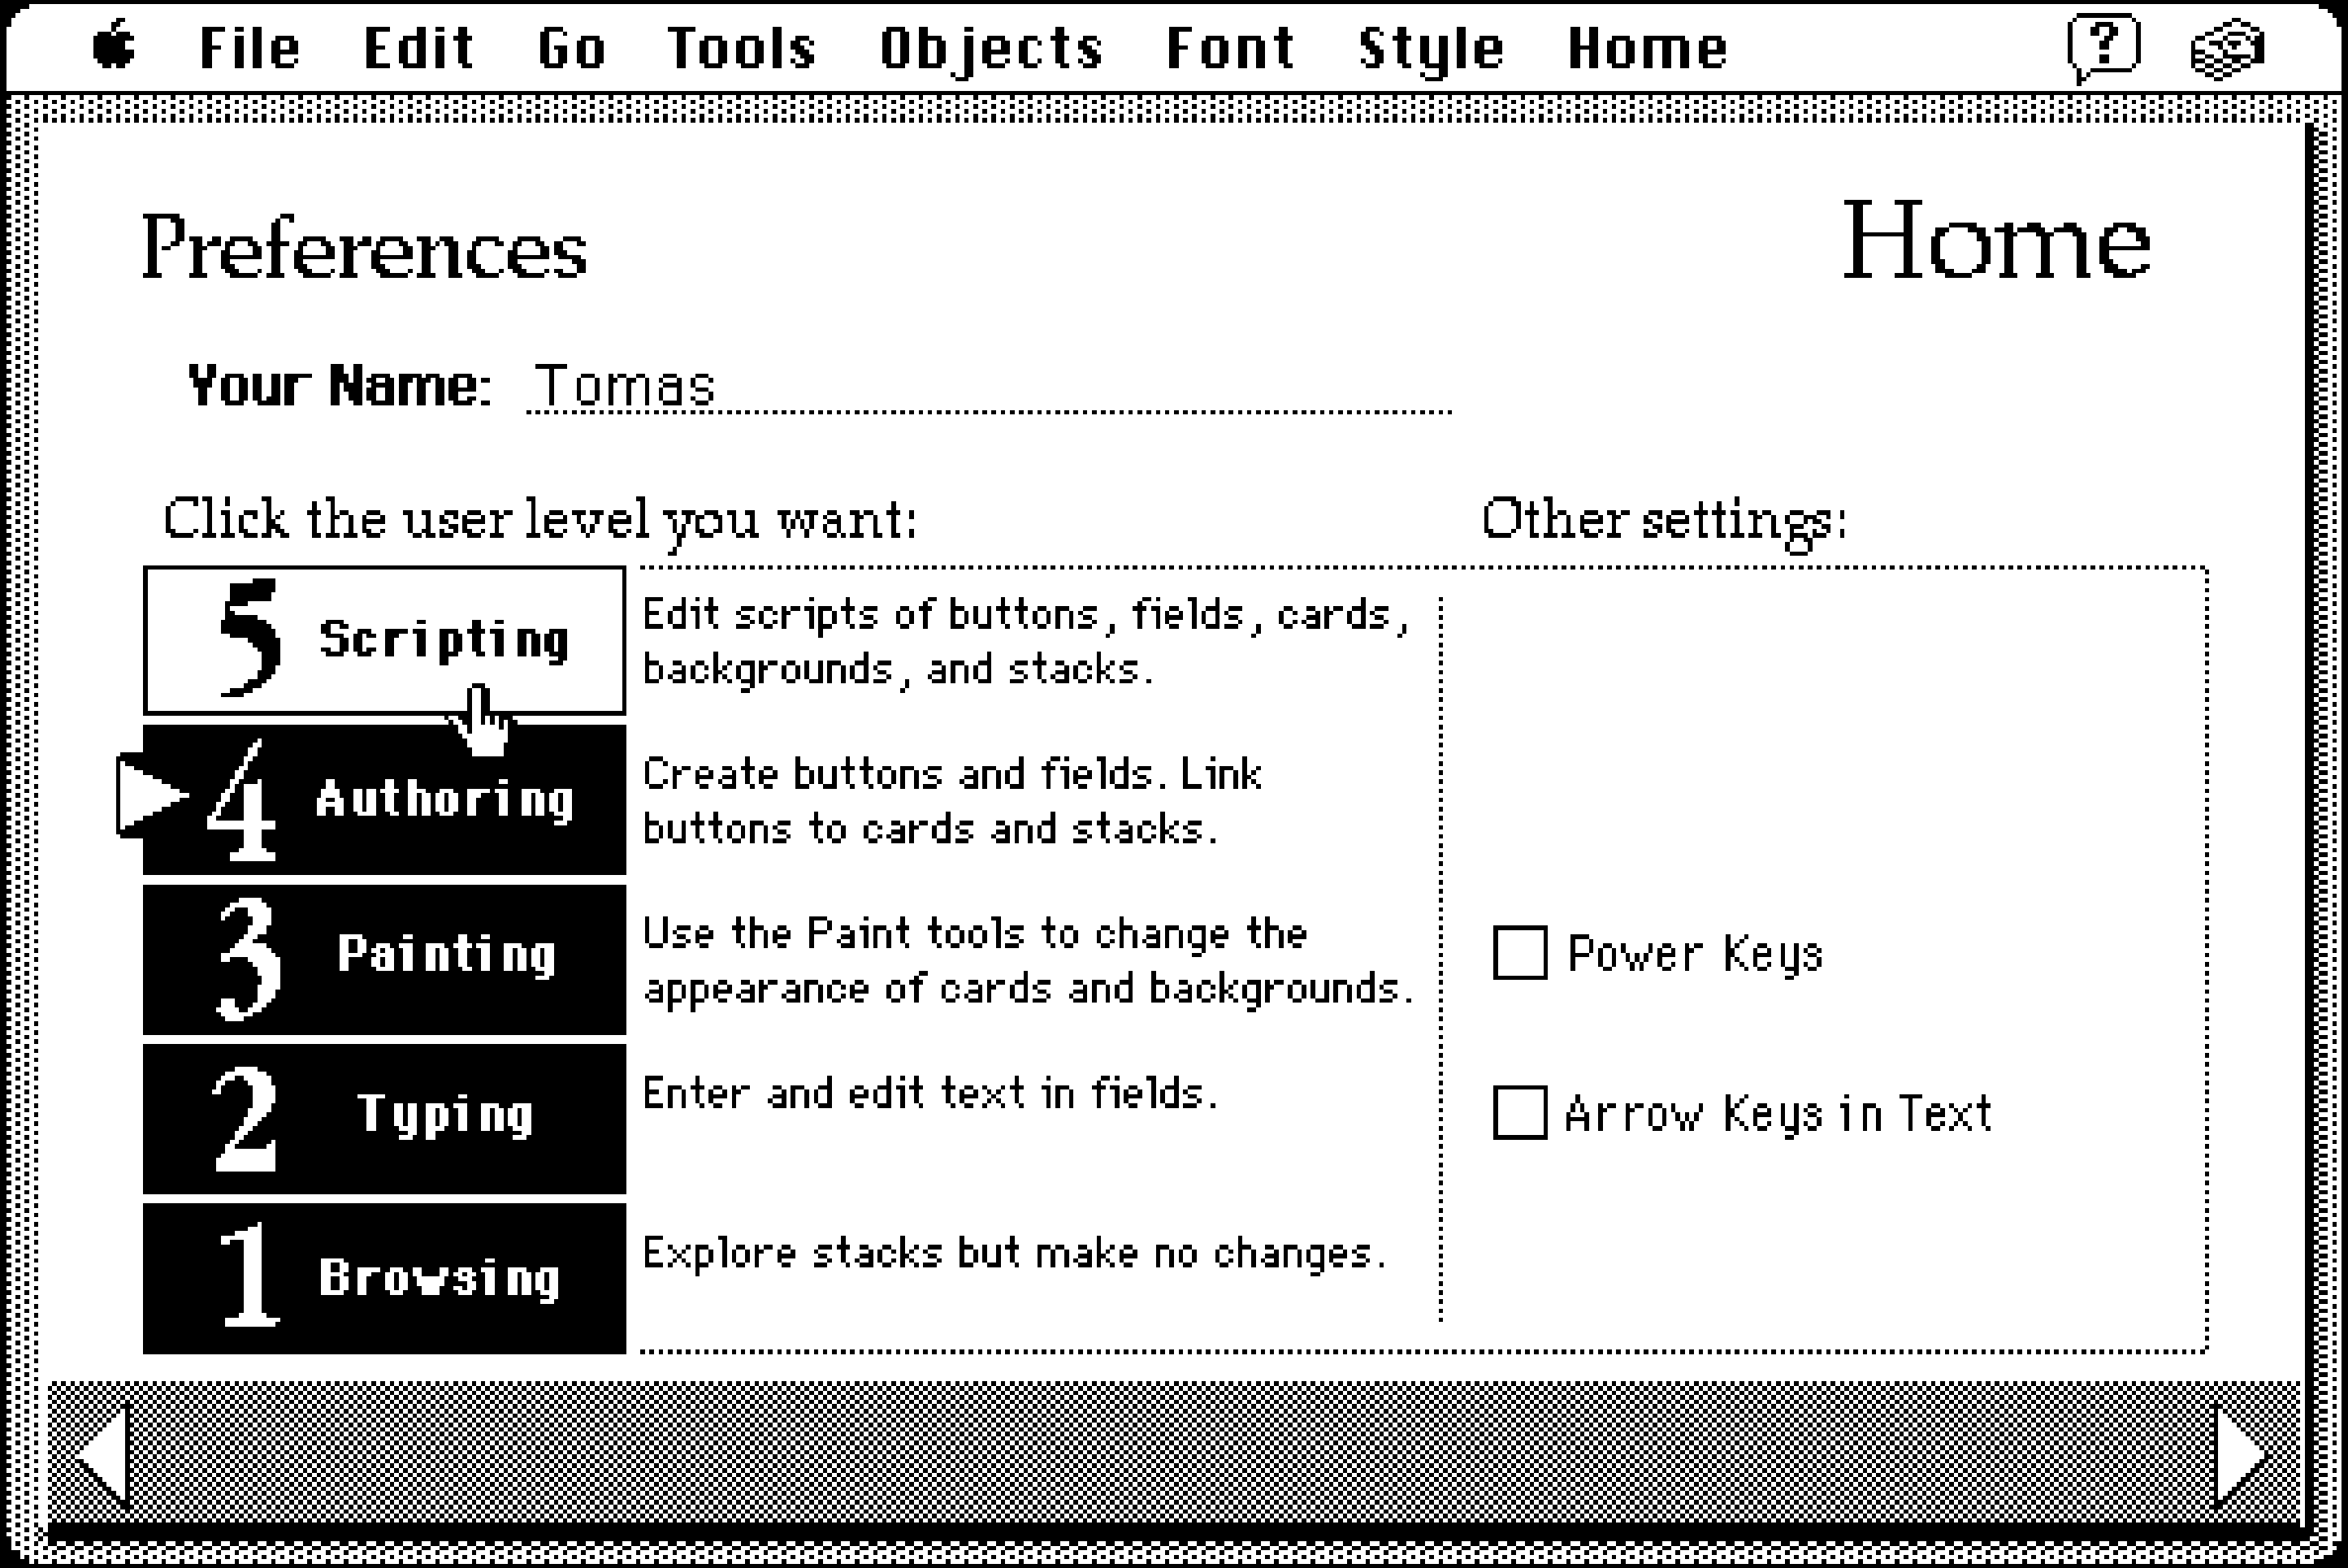
\includegraphics[width=0.6\textwidth]{fig/hypercard.png}
\caption{HyperCard preferences page, where the user can select a ``user level'' to change
the mode of interaction with a HyperCard program (screenshot by the author)}
\label{fig:hypercard}
\vspace{-0.5em}
\end{figure}

The design of HyperCard made it easy to copy, study and modify HyperCard stacks obtained from
other users and learn how to create new ones. It is worth noting that these characteristics
are remarkably similar to the two freedoms required by the Free Software Foundation.
I would thus argue that, just like BASIC on microcomputers was an unfaithful, but practical
realization of Alan Kay's Smalltalk vision, HyperCard was an unfaithful, but practical
realization of free software.

HyperCard stacks existed as local stand-alone files, which made them unsuitable for the
1990s era of the internet. The World Wide Web developed by Tim Berners-Lee
was also inspired by hypertext, but focused on sharing of information.
Reflecting its academic origins, the web was structured as interconnected set of
documents (rather than cards), but the documents also included other interface elements known from
HyperCard (like buttons). The fact that documents existed on public web servers, rather than
as local files, made editing a trickier problem. Despite some initial attempts, the World
Wide Web never allowed users to directly edit documents through the web browser. However,
the web remained open in the sense that users could view the source code of a web
page, save it locally, or copy parts of it for their own use. As I document later in this
article, the openness gradually disappeared. If a user opens a source code of a modern
web application, they no longer see comprehensible source code and have little chance
to understand what is happening with the data they enter.


\section{What is software openness}
\label{sec:openness}

Openness has been broadly defined as the ``accessibility of knowledge, technology and other
resources; the transparency of action; the permeability of organisational structures; and the
inclusiveness of participation.''\endnote{\citet{schlagwein-2017-openness}} In the context of
software, openness also manifests in different ways. The kind of openness of Free Software
differs from that of customizable end-user application such as HyperCard. We can separate the
two cases by distinguishing between the \emph{static openness} of the source code and documents
using which software system is produced and the \emph{dynamic openness} of the resulting
running software system.

\paragraph{Static openness}
The first kind of openness concerns the source code and other information about software.
The concept can be used for making a distinction between \emph{proprietary software} (information
about it is not available) and \emph{open source software} (the source code is available). Even
proprietary software can be closed to a varying degree. For example, different software development
methodologies recommend restricting access to particular information to different parts of the
development team. The notion is not restricted to source code. For example, an explanation of how
a key algorithm of a system operates, or a detailed description of collected data can be shared
in an accessible form with end-users.\endnote{Regulations such as GDPR can thus be seen as
requiring a minimal degree of openness of software.}

\paragraph{Dynamic openness}
The second kind of openness reflects the degree to which the structure of the (running)
software system is exposed. An application compiled to native code is dynamically closed
as it is difficult to reconstruct any information about its internal
structure.\endnote{As pointed out by \citet{kell-2019-lurking}, if an application is compiled with
suitable debugging information, it should still be possible to reconstruct its structure.}
Software systems that retain the original static structure are more open.
At an extreme end, a running Smalltalk system includes all class definitions with their source code,
allowing users to inspect and modify the running program. A more limited case is that of mobile
applications that need to access some device resource. The application needs to declare the
required permissions, which reveals (very little) information about its inner working.

\paragraph{Software opacity}
The two kinds of openness both contribute to the opacity of the
software we use today. If we face software that is both statically and dynamically
closed, we have no way of understanding how it operates. Dynamic openness makes software more
transparent to its end-users, while static openness serves primarily programmers.
In an open software system like Smalltalk the two notions partly overlap, because source code
becomes a part of the running system.

Each of the following two case studies focuses on one of these kinds. The discussion of
information sharing (\S\ref{sec:info}) is primarily concerned with static openness, while the
study of the web (\S\ref{sec:web}) emphasises dynamic openness.
As we will see, the decision making that is involved in choosing whether to make a
software system more open or more closed is very similar for both kinds of openness.

\section{Information sharing}
\label{sec:info}

Information hiding is a fundamental concept in computer science. Every student is taught to
design software in a way that hides the implementation details of a module, exposing only a
well-defined stable interface. The principle makes software more closed, but is accepted as a
good engineering principle. In the first case study, I retrace the origins and challenges of
information hiding.

\subsection{The OS/360 workbook}
In 1964, Frederick P. Brooks, Jr. became the manager of the IBM System/360 project, building a
newly designed family of computers. The operating system OS/360 designed for the computers
later became a well-known example of a software project completed late and significantly
over budget.\endnote{For an overview of the history of the IBM System/360 project, see the
article by \citet{cortada-2019-ibm}.} After leaving IBM, Brooks tried to answer the question of
why managing software projects was so difficult in his book \emph{The Mythical Man-Month}. The
reflections included the now so-called  Brooks' Law that ``adding manpower to a
late software project makes it later''. However, the book also discussed the problem of sharing
information.

Brooks believed that the ``problem is not to restrict information, but to ensure that relevant
information gets to all the people who need it.''\endnote{\citet[p.76]{brooks-1995-manmonth}}
According to Brooks, the view was supported by Harlan Mills, who argued that programming should be a
``public process'' and that ``exposing all the work to everybody's gaze helps quality control,
both by peer pressure to do things well and by peers actually spotting flaws and
bugs.''\endnote{\citet[p.271]{brooks-1995-manmonth}} The motivation for making information about the
software public (to all team members, although not necessarily its users)
was based on engineering and managerial reasons. Brooks and Mills were not concerned
with transparency or accountability, but with producing reliable software.

To ensure everyone has access to full information about the system, Brooks' team maintained
a project workbook containing \emph{``all} the documents of the project [including]
objectives, external specifications, interface specifications, technical standards, internal
specifications, and administrative memoranda.''\endnote{\citet[p.75]{brooks-1995-manmonth}}
The workbook was initially distributed on paper, eventually numbering over 10,000 pages.
Team members received updates of 150 pages daily that they had to add or replace in their
looseleaf copy of the workbook. This was tedious work, but it ensured that team members
were aware of the changes. The team later switched
to microfiche, which simplified maintenance, but meant that changes were no longer read.

\subsection{Information hiding}
A different way of thinking about information sharing was born only a couple of years later,
when David L. Parnas took a one year leav-of-absence from his academic post in 1969 to work with a
company in Netherlands and had a first-hand experience with software design that involved tight
coupling of components. When the ``control block format'' was changed by one team member, code
written by another team member that relied on the original format stopped
working.\endnote{\citet{parnas-2002-history}}

Initially, Parnas only had an intuition that the design was not ``beautiful'' in the same way
as, for example, Dijkstra's THE system.\endnote{\citet{dijkstra-1967-the}} Parnas first attempted to
analyze the problem in a paper \emph{Information Distribution Aspects of Design
Methodology} presented at the IFIP Congress in 1971.\endnote{\citet{parnas-1971-distribution}}
In the paper, he argues that information ``broadcasting'' that ``makes all information accessible
to anyone working on the project'' is harmful and that ``it is helpful if most system information
is hidden from most programmers.''\endnote{\citet{parnas-1971-distribution}}
Parnas illustrates the idea with a number of examples including I/O device addresses, character
codes, control block formats and memory maps.

In the following year, Parnas published two widely-cited journal papers,\endnote{\emph{On the
criteria to be used in decomposing systems into modules} \citep{parnas-1972-decomposing} and
\emph{A technique for software module specification with examples} \citep{parnas-1972-technique}}
in which he argues that a good design decomposes a system into modules that hide certain
information from other modules:

\begin{quote}
We propose (...) that one begins with a list of difficult design decisions or design decisions
which are likely to change. Each module is then designed to hide such a decision from the
others.\endnote{\citet{parnas-1972-decomposing}}
\end{quote}

According to Parnas, this approach leads to a more modular decomposition than the typical
approach of splitting system into subroutines based on a flowchart. The benefits
are:\endnote{\citet[p.2]{parnas-1972-decomposing}} (1) managerial, because teams can develop
modules independently; (2) greater flexibility, because modules can be changed independently; and
(3) comprehensibility, because modules can be understood one at a time.

Similarly to Mills and Brooks earlier, Parnas also makes the decision regarding information
sharing based on engineering and managerial reasons. He argues that information hiding will
make development faster and more flexible. Even comprehensibility is not framed as virtue on
its own, but as a practical benefit.

\subsection{The Mythical Man-Month, 20 years later}
When writing \emph{The Mythical Man-Month}, Fred Brooks was aware of Parnas' notion of information
hiding, but dismissed it as a recipe for disaster.

\begin{quote}
[Parnas has proposed that] the programmer is most effective if shielded from (...)
the details of construction of system parts other than his own. This presupposes
that all interfaces are completely and precisely defined. While that is definitely sound design,
dependence upon its perfect accomplishment is a recipe for disaster. A good information
system both exposes interface errors and stimulates their~correction.
\end{quote}

The \emph{$20^{th}$\,Anniversary Edition} of The Mythical Man-Month, published in 1995, includes
an additional retrospective chapter in which Brooks discusses which of the original ideas
still hold and which of his views have changed. Information hiding is perhaps the most notable
aspect of the original analysis where Brooks completely reversed his position:

\begin{quote}
I dismissed Parnas's concept as a ``recipe for disaster'' (...). Parnas was right, and I
was wrong. I am now convinced that information hiding, today often embodied in
object-oriented programming, is the only way of raising the level of software
design.\endnote{\citet[p.272]{brooks-1995-manmonth}}
\end{quote}

Brooks follows the admission with a more detailed analysis that, again, focuses on
engineering aspects of the decision. He notes that ``one can get disasters with either
technique,'' but concludes that a design based on information hiding is more appropriate
for designs that are expected to change.

\subsection{Free software}
The next contribution to the debate came from a more ideological
background. The members of the hacker culture, which formed at MIT at the end of the
1950s believed that ``all information should be free.''\endnote{\citet{levy-1984-hackers};
although, as pointed out by \citet{tozzi-2017-fun}, the actual history is more complex.}
At a time when most programming by the MIT hackers was done on two machines, this
meant that every programmer had access to everything on the machine, but the community also
later embraced ARPAnet, a predecessor of the modern Internet.

A more formal structure capturing the ideals of the hacker culture emerged in the 1980s
when Richard M. Stallman, referred to as ``the last of the true
hackers,''\endnote{\citet{levy-1984-hackers}} established the Free Software Foundation (FSF). The foundation
was established to support the development of the GNU operating system which was intended
as a replacement for the widely-used but non-free UNIX.\endnote{\citet{tozzi-2017-fun}}
The FSF initially viewed copyright and software license agreements as evil, but in the
late 1980s, Stallman and his colleagues realised that they could use copyright notice to
ensure that source code remains available for studying, copying and modification.
The version 1.0 of the license was issued in 1989. It captured the idea of free software that
was first described in the opening bulletin published by the Free Software Foundation in
1986. In the bulletin, Stallman explains that the word ``free'' in the name refers to a number
of fundamental freedoms:\endnote{\citet{stallman-1986-fsf}}

\begin{quote}
First, the freedom to copy a program and redistribute it to
your neighbors, so that they can use it as well as you.  Second, the
freedom to change a program, so that you can control it instead of it
controlling you; for this, the source code must be made available to you.
\end{quote}

In contrast to the writing of Brooks, Mills and Parnas who focus on managerial and engineering
values of information sharing (or hiding), Stallman's mission is rooted in the ideological
beliefs of the hacker culture.\endnote{\citet{petricek-2025-cultures}} Later in the bulletin, Stallman
describes the value of the GNU approach,\endnote{\citet{stallman-1986-arguments}} saying that ``user
who needs changes in the system will always be free to make them himself'' and that they ``will
no longer be at the mercy of one programmer or company which owns the sources and is in sole
position to make changes.'' However, Stallman also alludes to efficiency that would appeal to
managerially-minded Brooks and Mills when he points out that ``much wasteful duplication of
system programming effort will be avoided'' as the result of the openness.

\subsection{The cathedral and the bazaar}
Although the GNU source code was available for sharing and modification, the development
method employed by the GNU team was largely following the conventional
model based on a close collaboration of team members.
The increasing availability of computers connected over the Internet alongside with
the sharing of source code enabled a new development model to emerge in the 1990s.

The most prominent example of the new development model became the Linux kernel.
Linux started as a hobby project by Linus Torvalds, who was an undergraduate student in Finland
at the time. As documented by Tozzi,\endnote{\citet{tozzi-2017-fun}} Torvalds wanted to have a
fully-functional Unix-like operating system that would work on a PC. Torvalds was not
``much aware of the sociopolitical issues that were---and are---so dear to
[Stallman].''\endnote{\citet[p.51]{torvalds-2001-justforfun}} He was chiefly interested in having a system
that could run the tools developed as part of the GNU efforts at no cost.

Torvalds made his code available on the Internet, using a license that prohibited
commercial at first, but later switching to the GPL license. Living away from the large
computer science centres at the time, he started to remotely collaborate with numerous
volunteers, accepting patches and improvements.
Without realising it, Torvalds invented a new development model that relied on a large number
of loosely coordinated volunteers. A clear description of the revolution appeared a couple
of years later, in a paper presented by Eric S. Raymon at the Linux Kongress conference
in 1997 that was later published as \emph{The Cathedral and the
Bazaar}.\endnote{\citet{raymond-1997-cathedral}} As Raymond noted, the essay ``merely formalized
(...) what some FOSS developers (...) had been doing for years by that
point.''\endnote{\citet{raymond-1999-revenge}}

Interestingly, Raymond praises the ``bazaar'' development model of Linux not
because of its sociopolitical characteristics, but mainly because of its effectivity:

\begin{quote}
What I saw around me was a community that had evolved the most effective software-development
method ever and didn't know it! That is, an effective practice had evolved as a set of customs,
transmitted by imitation and example, without the theory or language to explain why the practice
worked.\endnote{\citet{raymond-1999-revenge}}
\end{quote}

Raymond's writing contains more references to the ideas of Fred Brooks than to those of
Richard Stallman. As pointed out by Frabetti,\endnote{\citet{frabetti-2014-theory}} the cathedral metaphor
in the title of the essay is itself a reference to Brooks, who likened the conceptual disunity of software to
those of Medieval cathedrals.\endnote{\citet[p.42]{brooks-1995-manmonth}} Raymond also grapples with
the constraints imposed by Brooks' Law. He argues that collaboration in a distributed fashion
reduces the need for communication, as well as its overhead, which was the root cause for the
delays described by Brooks. (Some 25 years later, developers of open-source projects suffering from
burnout as a result of toxic communication may yet again disagree with Raymond's
analysis.\endnote{\cite{raman-2020-stress}})

Raymond's essay embodies a shift from ideological arguments about information sharing
to those based on engineering and managerial reasons. He also moved away from
the term ``free software'' and started talking about ``open source'' as a more broader term
that includes software with licenses that do not enforce sharing of derivative works. To advocate
for his vision of open source, Raymond co-founded the Open Software Initiative (OSI). In a later
comment,\endnote{\cite{raymond-1999-shutup}} he clarified that he is all in favor of freedoms,
rights and principles supported by Stallman, but that the FSF tactics don't work whereas tactics
pursued OSI work. He argues that the Stallman's ``rhetoric is very seductive to the kind of people
we [hackers] are,'' but that the language ``simply does not persuade anybody but [hackers].''

The dispute between Stallman's ``free software'' faction and Raymond's ``open source'' faction
is explored in detail by Tozzi.\endnote{\citet{tozzi-2017-fun}} We can also see the dispute as a
clash between the more idealistic hacker culture and the more pragmatic engineering, or even
managerial cultures of programming.\endnote{\citet{petricek-2025-cultures}} The fact that open source
became a business strategy became evident in 1998 when Netscape announced that it would
open-source its web browser (which would later evolve into Mozilla Firefox). The decision was
inspired by Raymond's essay and its discussion of the merits of the ``bazaar'' development
methodology. Netscape had ``no deep-seated ideological commitment to the FOSS
movement.''\endnote{\citet{tozzi-2017-fun}} They saw the change in business terms, as a way to
``accelerate development and free distribution by Netscape (...) further seeding the market for
Netscape's enterprise solutions.''\endnote{\citet{tozzi-2017-fun}} In other words, engineering and
managerial reasons have, again, became the key factors for decisions regarding information
sharing in software.

\subsection{Beyond open source}
In the 2010s, the open source approach to software development has became the dominant
development methodology. Tozzi concludes his history of the free and open-source
software (FOSS) revolution by discussing the Android and Ubuntu projects, which ``are successful
when measured in terms of market penetration but have been perceived as failures by hackers who
do not see these initiatives as fulfillments of the true promise and potential of the
FOSS revolution.''\endnote{\citet{tozzi-2017-fun}} In recent years, the open source development
methodology has been embraced even by the fiercest former opponents of the free software
including Microsoft.

For the initiators of the free software movement, open source does not guarantee
the originally envisioned freedoms. It could be also argued that access to source
code in the modern computing context does not guarantee the ``freedom to change a program, so
that you can control it instead of it controlling you.''\endnote{\citet{stallman-1986-fsf}}
The access to source code may have been sufficient in the 1980s when most GNU users were other
computer hackers and the complexity of the system was moderate. Today, when large software systems
span millions of lines of code and the majority of their users has no programming experience,
the ability to ``change a program'' is merely hypothetical. This can be demonstrated, for
example, by the challenges faced by the soveregin mobile operating system initiatives by removing
dependence on Google from the open-source Android operating system.\endnote{\citet{grolleau-2021-mobile}}

\section{The closing of the Web}
\label{sec:web}

The World Wide Web was conceived by Tim Berners-Lee in 1989 at CERN.\endnote{\citet{gillies-2000-web}}
It was intended as a universal information sharing platform. The design of the web was inspired
by earlier projects that explored how computers could assist with information
sharing.\endnote{\citet{petricek-2025-cultures} associates many of the preceding developments with
the humanistic culture of programming.} For example, the concept of a hyperlink can be traced back
to the late 1960s work of Douglas Engelbart's on the oNLine System (NLS).

Many of the design decisions around the web that contributed to its openness were the results
of primarily engineering decisions. One example is the adoption of the Hypertext Markup Language
(HTML). Various markup formats were used before the birth of the web and many physicists working
at CERN preferred the more powerful \TeX system. As Gillies and Cailliau
point out, Tim Berners-Lee chose to use HTML to ensure that ``no matter what kind of computer you
had, an HTML page would be understandable, even if it didn't look exactly the same on all
computers.''\endnote{\citet[p.163]{gillies-2000-web}}

As an information sharing platform, the web was designed as an open system
and Tim Berners-Lee ``had long been an admirer of Richard Stallman.''\endnote{\citet{gillies-2000-web}}
Berners-Lee was aware of the Free Software movement and, inspired by the movement, released
the libwww library that implemented the core functions of the web technologies (including HTML
and HTTP) to public domain in 1992. Berners-Lee considered using the GPL license, but opted not
to, in fear that companies such as IBM would not use it.\endnote{\citet{kesan-2004-deconstructing}}
Berners-Lee admired Stallman's idealism, but he was also impressed
by the way he ``had harnessed the power of the geeks.''\endnote{\citet{gillies-2000-web}}
Arguably, the strategy proved correct and the number of web developers and users grew steadily.
The shift that made the web truly ``world wide'' occurred in 1993 when the Mosaic browser,
built at the National Center for Supercomputing Applications (NCSA), made the platform
available to anyone using a Macintosh or Windows computer.

\subsection{The rise of the vernacular Web}

In the 1990s, the web has escaped the realm of academic information sharing and
has developed a unique amateur culture that computer artist and historian Olia Lialina
documented in her essay \emph{A Vernacular Web}.\endnote{\citet{lialina-2009-web}}
According to Lialina, the early web ``was bright, rich, personal, slow and under construction.''
It was ``the web of the indigenous... or the barbarians.''\endnote{\citet[p.19]{lialina-2009-web}}

This unique culture developed, at least in part, thanks to the openness of the early web
technologies. These were the predecessors of fundamentally the same
technologies that are used on the web today, but they were used in a different way.
Web pages were written in plain HTML (Hypertext Markup Language). Like today, the web browsers
made it possible for users to view the source code of the web page, but as the web pages
were simpler, even amateurs could find their way through the markup.

Scripts that were used for adding interactive elements to the web pages were often embedded directly
in the web page (using the \texttt{<script>} tag) or they were included in linked JavaScript files
that the user could locate and inspect. The scripts were distributed in the same form in which they
were written and so an aspiring web creator could study, understand and modify them in the way
envisioned by the Free Software Foundation in the 1980s. As documented by Lialina:

\begin{quote}
Every element on the page, every line, figure, button and sound was on its own and could easily
be extracted, if not directly from the browser then from looking at the source code to find the
URLs of the files.\endnote{\citet{lialina-2009-web}}
\end{quote}

In other words, the early web exhibited dynamic openness. Web pages consisted of different
components (media files, scripts) and the structure of those components was accessible to
the web browser, but also to an interested user of the platform.
As documented by Lialina, this technological structure
enabled the development of the early vernacular web culture:

\begin{quote}
Consider the way early amateur websites were made. As clumsy as they might appear to trained
professionals, in terms of spreading the Internet’s architecture and culture, they were of huge
importance. In fact, the mental image we have of the medium today: intelligence on the edges of the
network, many-to-many communication, open source (even if it was just about how to use the
\texttt{<blink>} HTML tag), is the result of these early efforts.
\endnote{\citet{lialina-2009-users}}
\end{quote}

The decision of Tim Berners-Lee, to represent documents using an accessible markup format,
undoubtedly contributed to the rise of the 1990s web culture.\endnote{Even if the tag to make
text on the web page blink, reportedly conceived in a bar and implemented overnight, was only
added in 1994 \citep{montulli-2009-blink}.}

\subsection{Openness of the early Web}
At this point, it is useful to revisit the difference between the two kinds of openness analysed
in this article. The debate about information sharing (\S\ref{sec:info}) was mainly concerned with
human access to information, including source code and documentation. Information hiding started as
a merely organizational decision, but it later gained a technical meaning and evolved into a
programming language mechanism.\endnote{For this example, but also other cases where software
engineering had an effect on programming languages, see the review by \citet{ryder-2005-impact}.}
The Clu language implemented information hiding through a mechanism called \emph{abstract data
types},\endnote{\citet{liskov-1974-adt}} which ensured that programmers cannot, intentionally or
unintentionally, write code that accesses the hidden state of a component. In other words,
abstract data types hide the internal state of a component from the code that uses the component.

In the context of the web, we are concerned with information available dynamically, while the
server is running  and communicating with a web browser. For example, HTML documents that are
sent to the browser make their internal structure accessible. This appears inevitable---how else would
the web browser display the web page---but an alternative format focused on presentation
(such as PDF) can represent a document only as characters and their positions
on the screen, hiding the intent and the structure of the document from the application that displays
it. Furthermore, scripts that made the web interactive were also distributed in human-readable
source code format. They achieved many of their task by calling functions offered by the web
browser and, consequently, the structure and actions of a web page were transparent to the browser.
This architecture had interesting implications for one of the most hated artifacts of the 1990s
web---pop-up~ads.

\begin{figure}
\centering
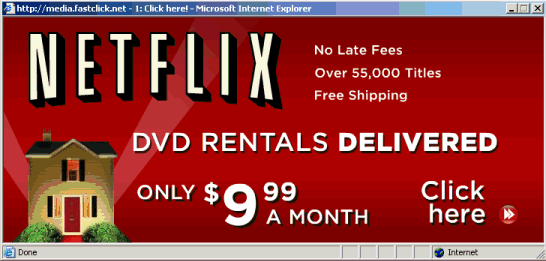
\includegraphics[width=0.7\textwidth]{fig/netflix.png}
\vspace{-0.5em}
\caption{Pop-up advertisement for Netflix DVD rentals, opened in a new web browser-managed window,
opened using \texttt{window.open} (from \citet{niedermayer-2019-ad})}
\label{fig:netflix}

\vspace{1em}
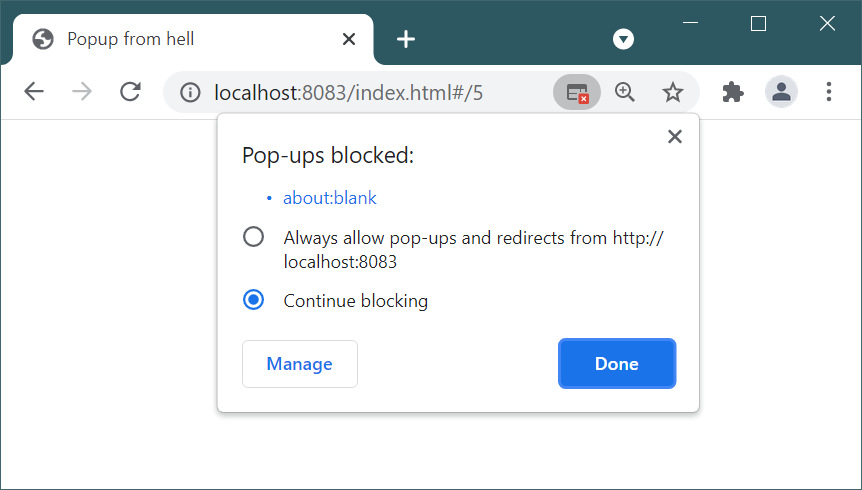
\includegraphics[width=0.7\textwidth]{fig/block.png}
\vspace{-0.5em}
\caption{An attempt to open pop-up window using \texttt{window.open}, blocked by the Chrome
web browser (screenshot by the author).}
\label{fig:block}

\vspace{1em}
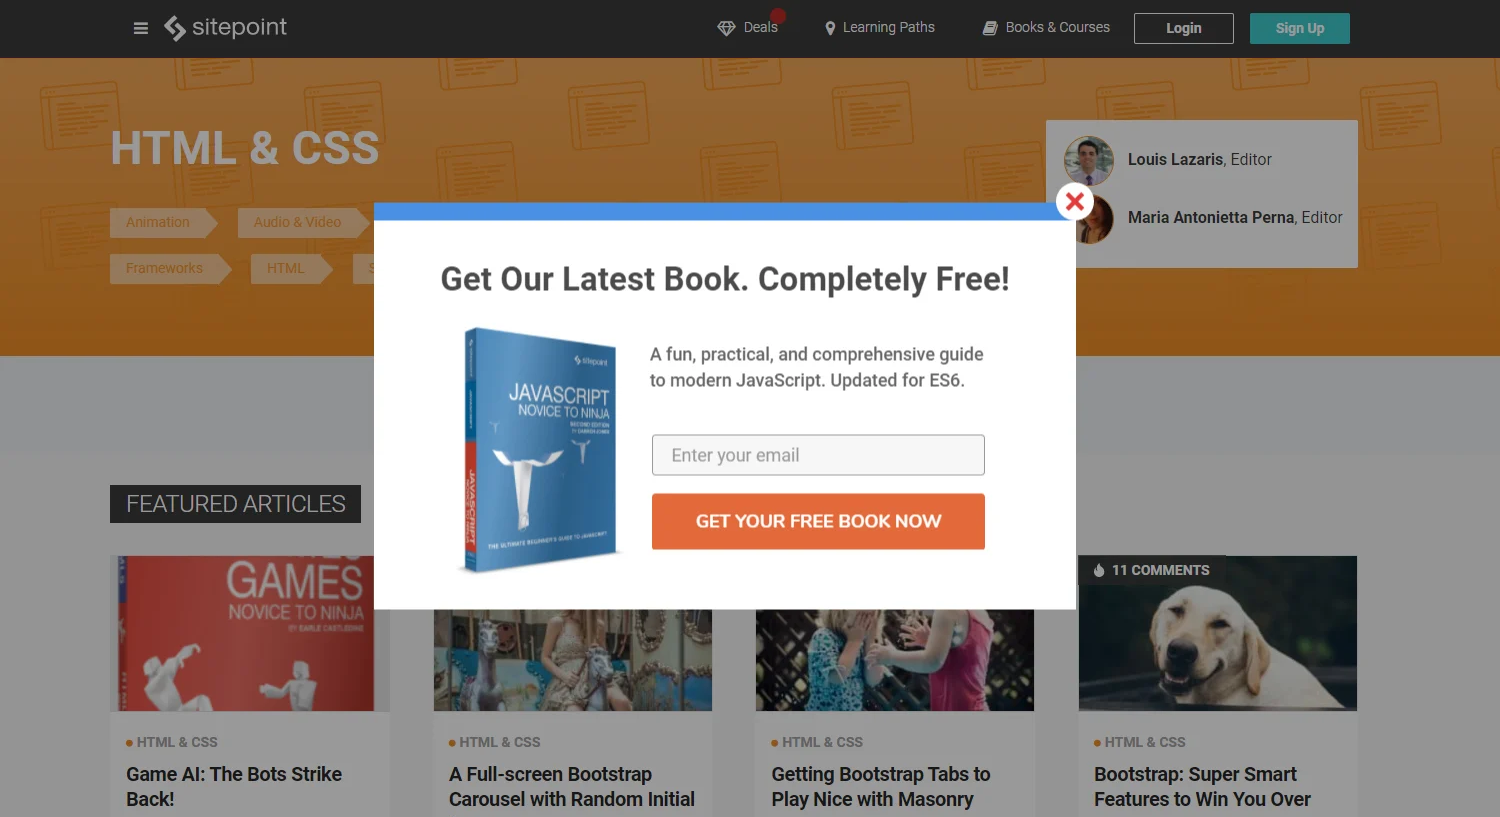
\includegraphics[width=0.7\textwidth]{fig/sitepoint.png}
\vspace{-0.5em}
\caption{An in-page pop-up ad, created using ordinary HTML elements within the content of the web
page, which is more difficult to detect and block (screenshot by the author).}
\label{fig:inpage}
\end{figure}

\subsection{Aside: Pop-up windows and ad blocking}

The pop-up ad (Figure~\ref{fig:netflix}) was created by Ethan Zuckerman at a web hosting company Tripod.com
in order to dissociate the advertisement from the web page content.\endnote{\cite{zuckerman-2014-sin}}
It relied on the \texttt{window.open} function that web browsers provided to scripts running
in the web page. The function could be called to open a new window with the specified content and
with the specified look (e.g., to remove the menu and the tool bar of the browser).

In the early 2000s, most web browsers developed techniques for automatically blocking pop-up ads
(Figure~\ref{fig:block}). Thanks to the transparency of the web, this was a relatively
easy task. The web browser only had to block calls to \texttt{window.open}, possibly with the
exception of calls directly triggered by some user interaction with the web site such as
clicking a button.

It did not take long for web developers who wanted to serve pop-up ads on their websites to
circumvent the restriction. Rather than opening pop-up ads using the \texttt{window.open}
function, which is provided and understood by the web browser, web developers re-created the
experience of pop-up ads using the standard HTML elements within the web page itself
(Figure~\ref{fig:inpage}). The behaviour of the web page is no longer transparent
to the web browser, which cannot easily block the advertisement. (Modern ad-blockers
can do so by recognizing specific patterns in the displayed HTML, but this requires a
detailed database of malicious~patterns.)

The story of pop-up ads is interesting, because it offers another perspective on the issue of
openness and information sharing in software. The early web sites with pop-up ads exhibited
dynamic openness with respect to the web browser. They exposed information about what
they were doing, which allowed the browser to handle various tasks on behalf of the web page
(such as opening a new browser window), but it also allowed it to prevent certain behavior.
In a commercially-motivated engineering move, developers of ad-supported web pages reimplemented
the functionality provided by the web browser in a way that made it less transparent.
As we will see, this kind of engineering-motivated closing of the web occurs repeatedly in more
recent history of the platform.

\subsection{Minification and obfuscation}
Following the economic dot-com bubble of the late 1990s, the web started to evolve into what
became labelled as Web 2.0, ``a phoenix arising from the ashes of dot-com design.''\endnote{\citet{ankerson-2018-dotcom}}
Web 2.0 was lauded as social, rich and user-driven. Some authors interpret Web 2.0 as primarily
a rhetorical move or a marketing term,\endnote{\citet{allen-2013-web20}} but the new use of the web
also relied on technological innovations developed throughout the late 1990s.
Web pages gradually evolved into interactive web applications, powered by increasingly
complex scripts. Technology known as Ajax made it possible for a web page to
retrieve further data from the server.

As a result of the new developments, the complexity of web applications was growing. They
included more JavaScript code and relied more heavily on the network. At the same time, most
users at the turn of the milenium still connected to the internet over a slow dial-up connection
and so downloading large JavaScript files could slow down the loading of a web page.
To address the issue, Douglas Crockford (later known for popularizing the JSON format) implemented
a tool called JSMin.\endnote{\cite{crockford-2019-jsmin}} The tool made JavaScript files smaller by removing
whitespace and comments from the source code. Although the transformation was relatively simple,
it meant that programmers now kept the original version of the source code to themselves
and distributed a less readable minified version of the code. In the ensuing quest for performance,
JavaScript minifiers became more sophisticated and started, for example, replacing longer local variable
names with shorter meaningless names (like \texttt{\_1}, \texttt{\_2} and so on).

The development of minification tools was largely motivated by engineering reasons. Their
purpose was to make the growing JavaScript files smaller. But as a side effect, they also made
the web more closed. Viewing the web page source code no longer displayed a version of the
code that the reader could study, understand and modify. In other words, the web lost its dynamic
openness, where a readable source code of the web page was accessible to all users. Making a
web page statically open, by sharing the non-minified source code, became decision that had
to be made consciously and explicitly.

A parallel ideologically motivated move was the development of tools, later known as obfuscators,
which prevented users from viewing the ``programming tricks'' behind the increasingly complex web
applications. One of the earliest attempts was the Script Encoder developed by Microsoft in
1999.\endnote{Script Encoding was a feature of the Microsoft Script Engine Version 5.0
\citep{clinick-1999-scriptenc}.} An article introducing the tool opens with a catchphrase ``Tired
of exposing your Web scripting code to prying eyes?'' and then goes on to explain the motivation:

\begin{quote}
[The popularity of scripting has also] been accelerated [by] the ability to see what
programming tricks others have employed simply by loading a page into Notepad. While this is a
great asset for the beginning script programmer, people who are developing increasingly complex,
script-based applications want to be able to protect their hard work.
\end{quote}

Unlike with minification tools, the Script Encoder was built to
protect intellectual property -- the announcement talks about ``pros\-pective pirates''
and ``illegal copying''. Technically, script encoding transformed Java\-Script code into an
opaque sequence of characters. The only way to run encoded scripts was to use Internet Explorer 5.0,
which was able to decode them, and so the technology also forced users to adopt Microsoft's web browser.

Script Encoder was soon reverse engineered and its dependence on Internet Explorer 5.0
further limited its applicability, but the desire to hide the source code soon came together with
the desire to reduce file size. More sophisticated minifiers made the source code difficult to
restore because they renamed variables or even compressed (and reconstructed at runtime) the stream
of JavaScript tokens.\endnote{This approach was used by Dean Edwards' Packer \citep{akulov-2025-packer}.}
Perhaps because the two goals were served by a technically similar tool, many systems of the
mid-2000s claimed they serve both purposes. The Free JavaScript obfuscator claimed
that it ``protects JavaScript code from stealing and shrinks size.''\endnote{\citet{cutesoft-2005-obfuscator}}

\subsection{Web application development}

Another issue with the increasingly complex Web 2.0 applications was that they had to be
written in JavaScript. The language became widely used because it was available in most web browsers,
but it was generally regarded as a poor engineering tool. The opening chapter of a book
\emph{JavaScript: The Good Parts}\endnote{\citet{crockford-2008-goodparts}} written by the creator of
JSMin, Douglas Crockford, illustrates the common perception (before offering a somewhat more positive
view of the language):

\begin{quote}
JavaScript is a language with more than its share of bad parts. It went from non-existence
to global adoption in an alarmingly short period of time. It never had an interval in the lab
when it could be tried out and polished. (...) JavaScript's popularity
is almost completely independent of its qualities as a programming language.
\end{quote}

Crockford also explains that JavaScript is not the only problem with web application development.
Another issue is the design of the Document Object Model (DOM), an API through which JavaScript
applications control the web page and the browser. The DOM is ``quite awful,'' as well as ''poorly
specified and inconsistently implemented.''\endnote{\citet[p.2]{crockford-2008-goodparts}}

Given this perception of JavaScript and DOM, it is perhaps not a surprise that software engineers,
as well as many academic researchers started to look for better tools.\endnote{Early academic
programming languages that targeted JavaScript included, for example, those by
\citet{cooper-2007-links,petricek-2007-webtools,serrano-2006-hop}.}
One of the first large-scale frameworks that aimed to turn
web application development into proper engineering was the Google Web Toolkit (GWT).\endnote{\citet{gwt-2006-gwt}}
The toolkit was created as a web development framework based on the Java programming language.
Programmers would create web applications in Java (instead of JavaScript), using a library of
GWT user interface components (instead of the DOM) and the toolkit would translate their code
to JavaScript, so that it can run in the web browser. The engineering motivation behind the
system can be illustrated by looking at the GWT home page from 2006. It included a typical
critique of the web ecosystem at the time (quoting JavaScript's lack of modularity, browser
quirks and incompatibilities) and outlined a range of engineering benefits of the Java language
as an alternative (advanced development tools, static type checking, object-oriented design).

The Google Web Toolkit emerged as a reasonable engineering response to the challenges posed by Web 2.0
application development. It enabled developers to use a more robust and modular programming
language, provided libraries that hide incompatibilities between web browsers and offered sophisticated
debugging tools (which run the code directly as Java in a special web browser). At the same time,
the translation to JavaScript, alongside with the increasingly complex abstractions, contributed
to the closing of the web. The users could no longer easily locate source code for components of
the web page. The aim of protecting source code from copying was not explicit in the design
of GWT, but it was a side effect of the engineering design choices. The web of the late 2000s
was no longer  ``the web of the indigenous... or the barbarians.'' It was the web of
professional software engineers.

~

The trend started by JSMin and the Google Web Toolkit continues to the present day. Multiple new
programming languages that aim to improve on Java\-Script have emerged, including CoffeeScript, Dart
and, more recently, the widely adopted TypeScript language released by Microsoft in 2012. Most JavaScript code
distributed to the web browser is transformed by a ``bundler'' such as WebPack that combines
source code from individual modules into a single minified file.

The choice to distribute translated and minified code to the web browsers had multiple consequences.
The fact that users could no longer study and copy code was not a concern for the new class of
professional web developers. However, the choice also made it hard to debug scripts. When an error
occurred, the browser could only display the unreadable minified source code.  This fact inspired
the development of Source maps,\endnote{\citet{takikawa-2024-sourcemap}} a standard that describes mapping
of the generated JavaScript code back to the original source code.
This is noteworthy because it shows how an original desirable characteristic of
the open web got lost in a later engineering-motivated technical development, only to be
expensively recovered in the new context.

\subsection{From canvas rendering to Web Assembly}
Two even more recent developments within the web platform again illustrate the same pattern,
where a desirable characteristic of the open web gets lost as an unintended side-effect
of engineering-motivated technological development. The first development is best illustrated
through the story of Google Docs.

In May 2021, Google announced that it will be changing how Google Docs, their online word processor,
renders documents.\endnote{The original announcement is available from Google's blog
\citep{google-2021-canvas}.} Before, the documents created by the users were represented as HTML elements
on the page. As the user edited the document, Google Docs modified the HTML elements through the
DOM interface provided by the web-browser. According to the announcement, this approach was
inefficient and had inconsistent results as different browsers rendered documents slightly
differently. To have more control over rendering of documents, Google instead decided to implement
their own rendering using the \texttt{<canvas>} HTML element. This way, the Google Docs
engine would render the document into a bitmap and then display the bitmap on the web page.
This gave Google programmers full control of the rendering process, but it makes the document
entirely opaque to the web browser. Instead of a tree of HTML elements containing the text
written by the user, the browser only sees a single \texttt{<canvas>} element.

The announcement raised a number of concerns, the most notable being about accessibility.\endnote{\cite{macmanus-2021-canvas}}
Screen readers and other accessibility tools rely on the DOM to access the text on the page
or change visual settings. This is no longer possible if all the text exists only in a bitmap.
To recover assistive technologies, Google Docs engineers had to add an option to render the
document as ordinary HTML elements, invisible to the end-user, but accessible to the
screen readers.

At the same time, some engineering-minded commentators saw the move as a step towards
``an app-focused future'' of the web where canvas-based rendering ``centralizes the power in the
hands of the app.'' The openness of the web that used to make it possible to examine the
document structure ``may be nothing more than a brief and transient anomaly in the history of
software design.''\endnote{\cite{macdonald-2021-canvas}}
In many ways, the development mirrors the earlier temporary move from the open HTML-based
web pages to closed web applications built using the Flash multimedia platform in the 2000s. The
inaccessibility of applications built using Flash was also one of the frequently criticised
aspects of the move.\endnote{\citet{ankerson-2018-dotcom}}


The second recent development is the increasing adoption of Web Assembly, a technology
that was announced in 2015 and became a web standard in 2019.\endnote{\cite{w3c-2019-wasm}}
Web Assembly is a low-level, binary instruction format designed to run high-performance
code in a web browser at a speed on par with native code. Web Assembly aims to replace
JavaScript as the compilation target for compilers that make it possible to run code
written in other languages in the web browser including C/C++. The motivation for Web Assembly
was primarily an engineering one---to be able to run high-performance low-level code
in the web browser and compile existing libraries in languages like C/C++ for the web.
Yet, like many other developments discussed in this section, it contributes to making
the web even more opaque. Instead of seeing JavaScript code you could study, understand
and modify, you will be seeing low-level assembly-like instructions.\endnote{For debugging
purposes, Web Assembly supports source maps, and so developers may see their original
source code in the web browser, but source maps will most likely not be distributed with the
finished web application.}


\begin{figure}
\centering
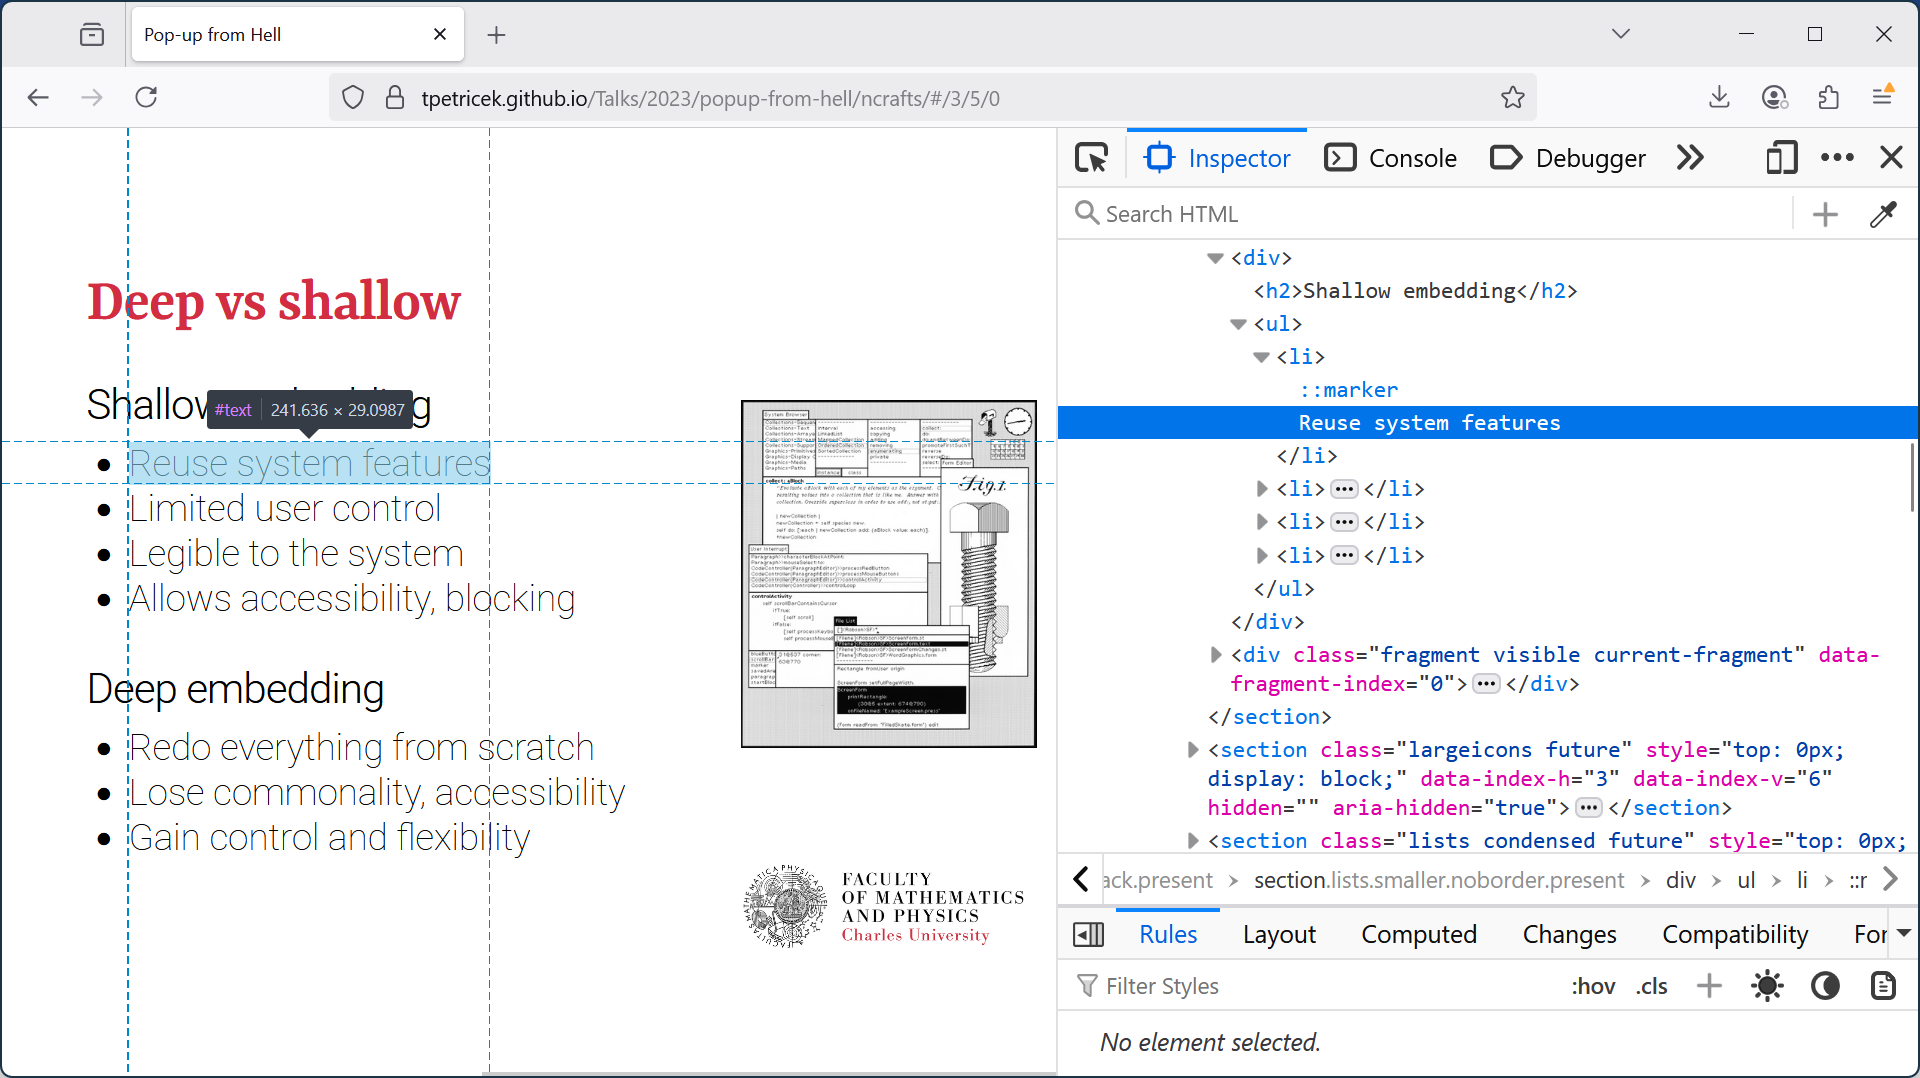
\includegraphics[width=0.95\textwidth]{fig/embedding.png}
\caption{A web page (talk slides) displayed in the Firefox Web Developer
Tools, showing the HTML structure of the page with the raw text (screenshot by the author).}
\label{fig:embedding}
\end{figure}

\subsection{Deep and shallow embedding}
Many of the engineering decisions in the history of the web can be framed in terms of
\emph{embedding}. Practically all software running on a computer is embedded in a
system that exposes services and provides information that the software can use.
A native program or a mobile app runs embedded in an operating system that controls
its access to resources and provides it with services that the application can use,
for example to display a user interface or manage files. In the case of a web applications,
the browser is the system. It provides the object-oriented JavaScript programming
model, access to the document through the DOM and rich rendering capabilities for displaying
text, user interface elements and styling them with CSS.

A web application can choose to leverage as many of those system capabilities, or it may
choose to rely only on a small necessary set of core primitives. An application that uses
\emph{shallow embedding} reuses as many system features as possible. This makes the application
legible to the system and, through the system, possibly also to the end-user. For example,
a web application that uses the DOM and CSS for its graphical interface makes the structure
of its interface visible to the system. The web browser can display the structure through
web browser development tools to the end-user (Figure~\ref{fig:embedding}) and the structure
is also accessible to browser extensions such as ad-blockers. Similarly, if a web page uses
the system-provided \texttt{window.open} function to open a pop-up window, the behaviour can
be easily recognized by the system and (possibly) blocked.

An application that uses \emph{deep embedding} relies only on minimal set of functions
provided by the system. In the aforementioned case of Google Docs, the developers choose
to rely on canvas-based rendering (that lets them display a bitmap) and re-implement all
the necessary text layout algorithms that are needed to display a document. The Flash
multimedia platform allowed users to run applications within a web browser, but without
leveraging any of the services provided by the browser. Similarly, many compilers
 that target JavaScript (or Web Assembly) may ignore much of the object-oriented
programming capabilities provided by JavaScript and produce code that re-implements much
of what the web platform already provides.\endnote{The degree varies depending on the
language. For example, TypeScript intentionally reuses much of JavaScript's programming model,
while the ghcjs compiler for Haskell (\url{https://github.com/ghcjs/ghcjs}) reimplements
the Haskell semantics including lazy evaluation and the resulting programming model is
very different from the JavaScript one.}

As the historical examples discussed in the preceding section show, developers often choose
deep embedding for engineering reasons. Deep embedding provides a greater control of how
the software is developed and how it can operate. Software engineers can use a programming
language with their preferred semantics (different from the JavaScript one), they can
create custom graphical user interfaces (changing the look of a pop-up or a drop-down control),
or they may implement certain functionality more efficiently. However, the cost of deep embedding
is the growing opacity of the resulting software.\endnote{Arguably, software engineers often
think they can do better than the system developers. This may be the case if the system
functionality is more general than the functionality needed by the software engineers in
a more specific case.} The software stops being legible to the system, accessibility tools
and also to the end-users.

\begin{figure}
\centering
\vspace{-1em}
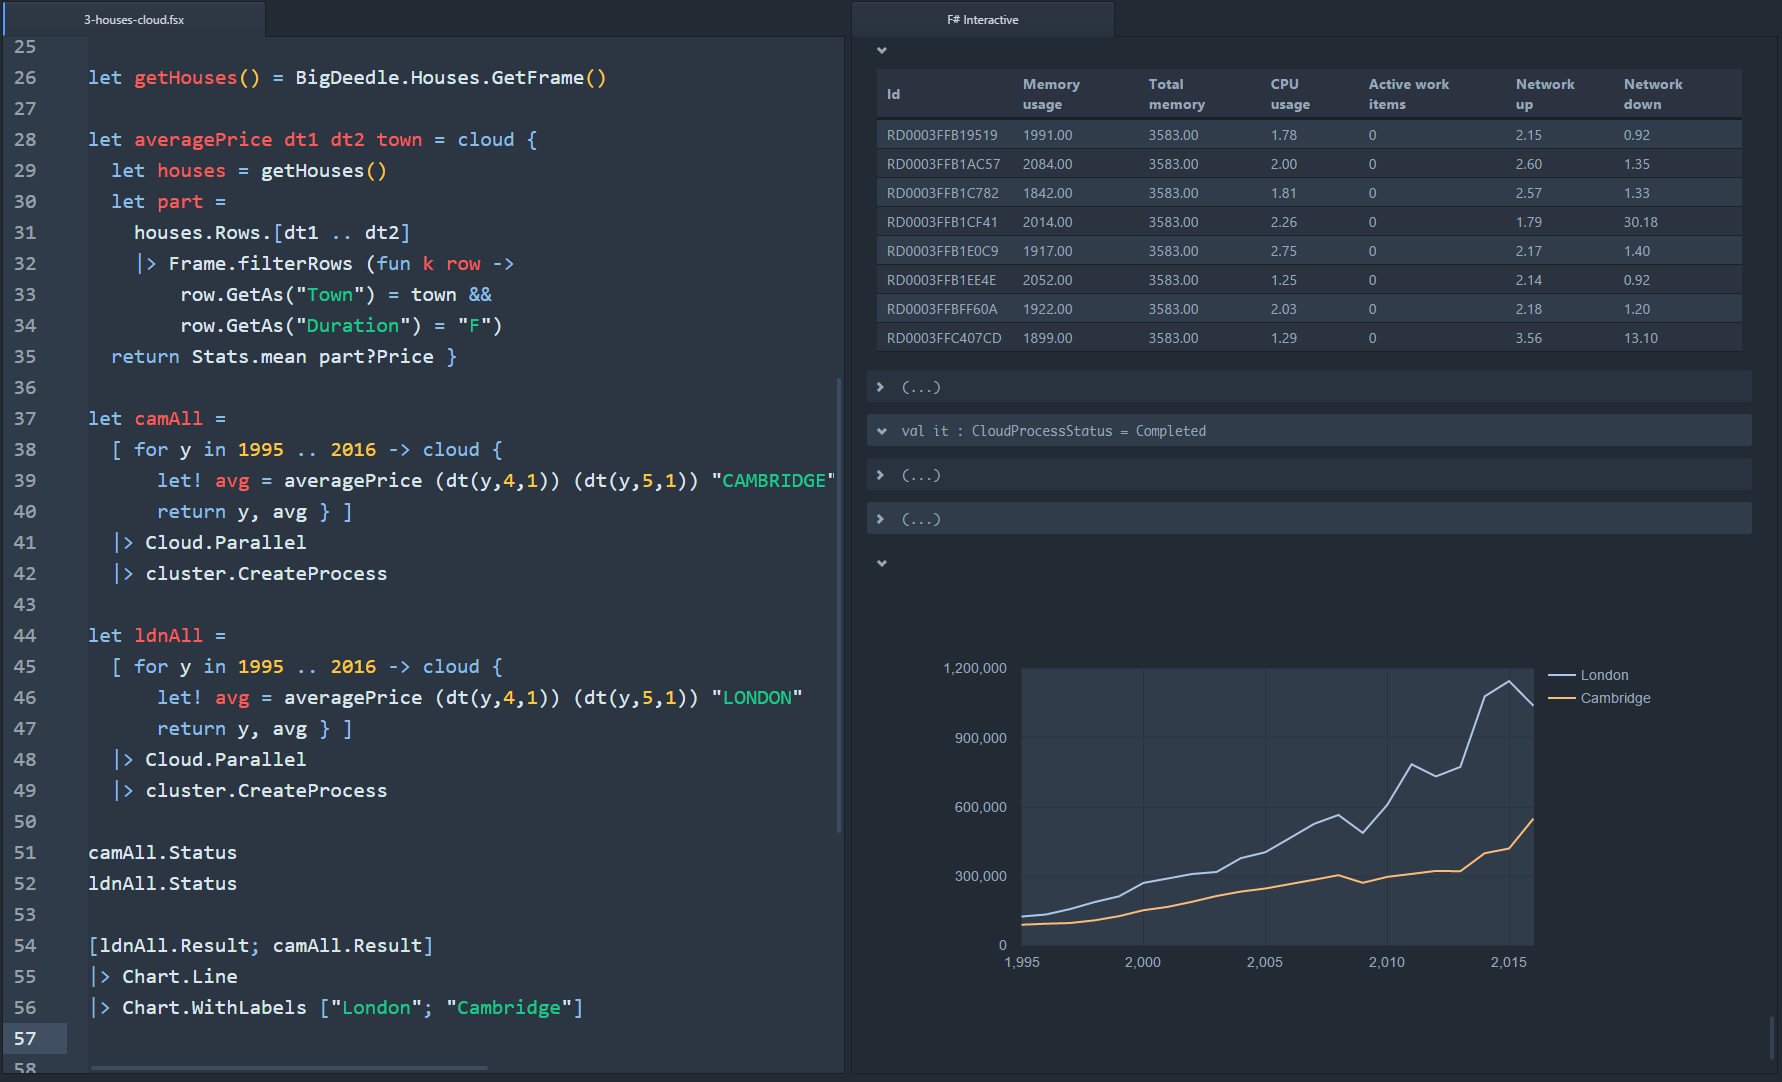
\includegraphics[width=0.86\textwidth]{fig/atom.png}
\caption{Analysing data with the FsLab extension for Atom. The right panel shows the status
of a cluster running the computation and a resulting chart (from \citet{petricek-2016-fslab})}
\label{fig:atom}
\end{figure}

\section{The editor wars of the 2000s}
In the previous two sections, we have seen how well-intended engineering decisions contribute
to the closing of software. To see that the two case studies illustrate a common scenario,
it is worth looking at one more example.

In 2015, GitHub released its open-source text and code editor called Atom. The editor was developed
in JavaScript and leveraged the Electron platform to run as cross-platform desktop
application.\endnote{In reality, Atom was built using CoffeeScript, which is a lightweight
programming language that compiles to JavaScript and simplifies its syntax.}
Atom was touted as ``a hackable text editor for the 21st century''.\endnote{The wording can
still be found in the project repository: \url{https://github.com/atom/atom}.}
The slogan reflects an important design decision in the Atom editor architecture.
The user interface of the editor was based on the web platform and the Electron platform
uses the web browser to display it.\endnote{More specifically, Electron is based on the
Chromium web browser, which is the core version of Google Chrome.}

The Atom user interface is represented using the DOM and it is accessible to editor extensions.
This means that any extension can access the user interface and even make changes to it.
The design is fragile as a faulty extension can break the user interface. But the design also
makes the editor flexible. This ``hackability'' allowed the Atom community
to create extensions that extended and modified the user interface in practically useful
ways, unanticipated by the original Atom developers. For example, the FsLab package
(Figure~\ref{fig:atom}) extended Atom with data visualization tools capable of loading
large data sets on-demand.\endnote{\citep{petricek-2016-fslab}}

Only a year after Atom became available, Microsoft released its own cross-platform open-source text
and code editor project called Visual Studio (VS) Code. Microsoft's editor was also based on
Electron and the web platform. It was written in TypeScript and compiled to JavaScript.
However, its approach to extensibility was very different
from Atom. VS Code was described using a somewhat nondescript tagline ``Code Editing.
Redefined,''\endnote{Posted on \url{https://code.visualstudio.com} in 2015
(\href{https://web.archive.org/web/20150903232639/https://code.visualstudio.com/}{archived}).
The tagline has since been replaced with ``The open source AI code editor''.}
but a part of its messenging was that it is efficient and reliable.
This was reflected by its approach to extensions:

\begin{quote}
Extensions are wonderful but extensions can also affect startup performance or the overall
stability of VS Code itself. To avoid these problems, VS Code loads and runs extensions in
a separate process, the extension host process. A misbehaving extension cannot impact VS Code
and in particular its startup time.\endnote{Available from
\url{http://code.visualstudio.com/docs/extensions/our-approach} in 2016
(\href{https://web.archive.org/web/20160814143739/http://code.visualstudio.com/docs/extensions/our-approach}{archived}).}
\end{quote}

In other words, VS Code does not allow extension authors to directly manipulate the DOM.
They can only communicate with the editor through an API that provides limited and controlled
access to the editor.

The logic behind the decision follows the one we have repeatedly seen earlier. The more flexible
open design that allows users to modify the software is interpreted as a poor engineering decision
that affects qualities of the software that an engineer may value, such as performance and
stability. An alternative design resolves the engineering issue, but also limits the flexibility
of the system. Being aware of the more open alternative, VS Code users repeatedly ask for
customizations that were doable with a small tweak to a ``user stylesheet'' or a ``user script''
in Atom.\endnote{See the GitHub issue on the  topic:
\url{https://github.com/microsoft/vscode/issues/459}.} Many of those customizations
are slowly added to the official VS Code configuration and supported extension API, but the
core design of VS Code remains closed. Even the existence of an open alternative
has thus served as a source of ideas for the closed software system.

In the case of VS Code, managerial decisions combined with engineering decisions to
provide a post-script to the story. Microsoft acquired GitHub in 2018 and despite initial
claims not to do so, discontinued the development of Atom.\endnote{See the post
\emph{Sunsetting Atom}, published on the GitHub blog in 2022:
\url{https://github.blog/news-insights/product-news/sunsetting-atom/}}

\section{Beacons of openness}
\label{sec:beacons}

If the closing of software is the result of engineering and managerial decisions, then
one way through which a more open software could be realised is by using designs that
justify openness not through ideological visions, but through managerial and
engineering reasons.

An engineering argument in favor of openness has been made by Clark and Basman, who
point out that the longevity of the MIDI interface for controlling devices
such as synthsizers or drum machines has largely been due to its
opennness.\endnote{MIDI devices expose their state through semi-conventionalized system
exclusive (SysEx) messages \citep{clark-2017-gpii}.} According to conventional wisdom,
such systems may appear as workarounds or quirks, but a more careful examination reveals
their engineering value.\endnote{Looking at the history of science in order to recover
valuable past ideas that have been forgotten is the aim of the \emph{complementary science}
methodology developed by \citet{chang-2004-temperature}.}

\subsection{Retrofitting openness}

Kell's analysis of Unix systems draws a distinction between ``application''
programming and ``device'' programming.\endnote{\cite{kell-2019-lurking}} In the former,
the program is a binary executable that runs as a process and keeps state in its own memory,
using its own file formats for persistent storage. In the latter, the program is a
collection of shell scripts that manipulate files in human-readable text format.
The two approaches correspond directly to deep and shallow embedding as discussed in this article.

In application programming (deep embedding), the memory structure and file formats are opaque
to the system, other applications and the user. In device programming (shallow embedding), the
state stored in text files can be shared across applications, inspected and even modified by the user.
This openness is, arguably, one of the reasons for the success of the Unix
programming philosophy\endnote{The philosophy, outlined by \citet{mcilroy-1978-foreword},
includes ``make each program do one thing well'' and ``expect the output of every program to
become the input to another, as yet unknown, program.''} and an engineering reason for
applying the philosophy more broadly.

There are two directions through which software on wide-spread Unix-like systems
(including Linux, Mac and Windows) could become more open. A direction recently outlined by
Jakubovic\endnote{\cite{jakubovic-2025-smalltix}; an earlier work going in a similar direction
explored the idea of using directories as files \citep{wimmer-2018-fad}} is to build more programs
on top of the Unix device programming model. His Smalltix project sketches how an object-oriented
programming model could be mapped to Unix device programming, enabling, for example, inspectable and
composable GUIs. The other direction is to make Unix application programming more like device
programming. Kell outlines how this could be done using the Smalltalk-like capabilities
lurking inside Unix.\endnote{\citet{kell-2013-lurking}; one example is the \textsc{Dwarf}
format for recording debugging information, which can be seen as a lurking Smalltalk metasystem.}
He argues for ``building a Smalltalk \emph{out of} the fragmented reality of today's Unix systems,
rather than running isolated Smalltalks (...) each trapped \emph{within} a Unix''.

\begin{figure}
  \centering
  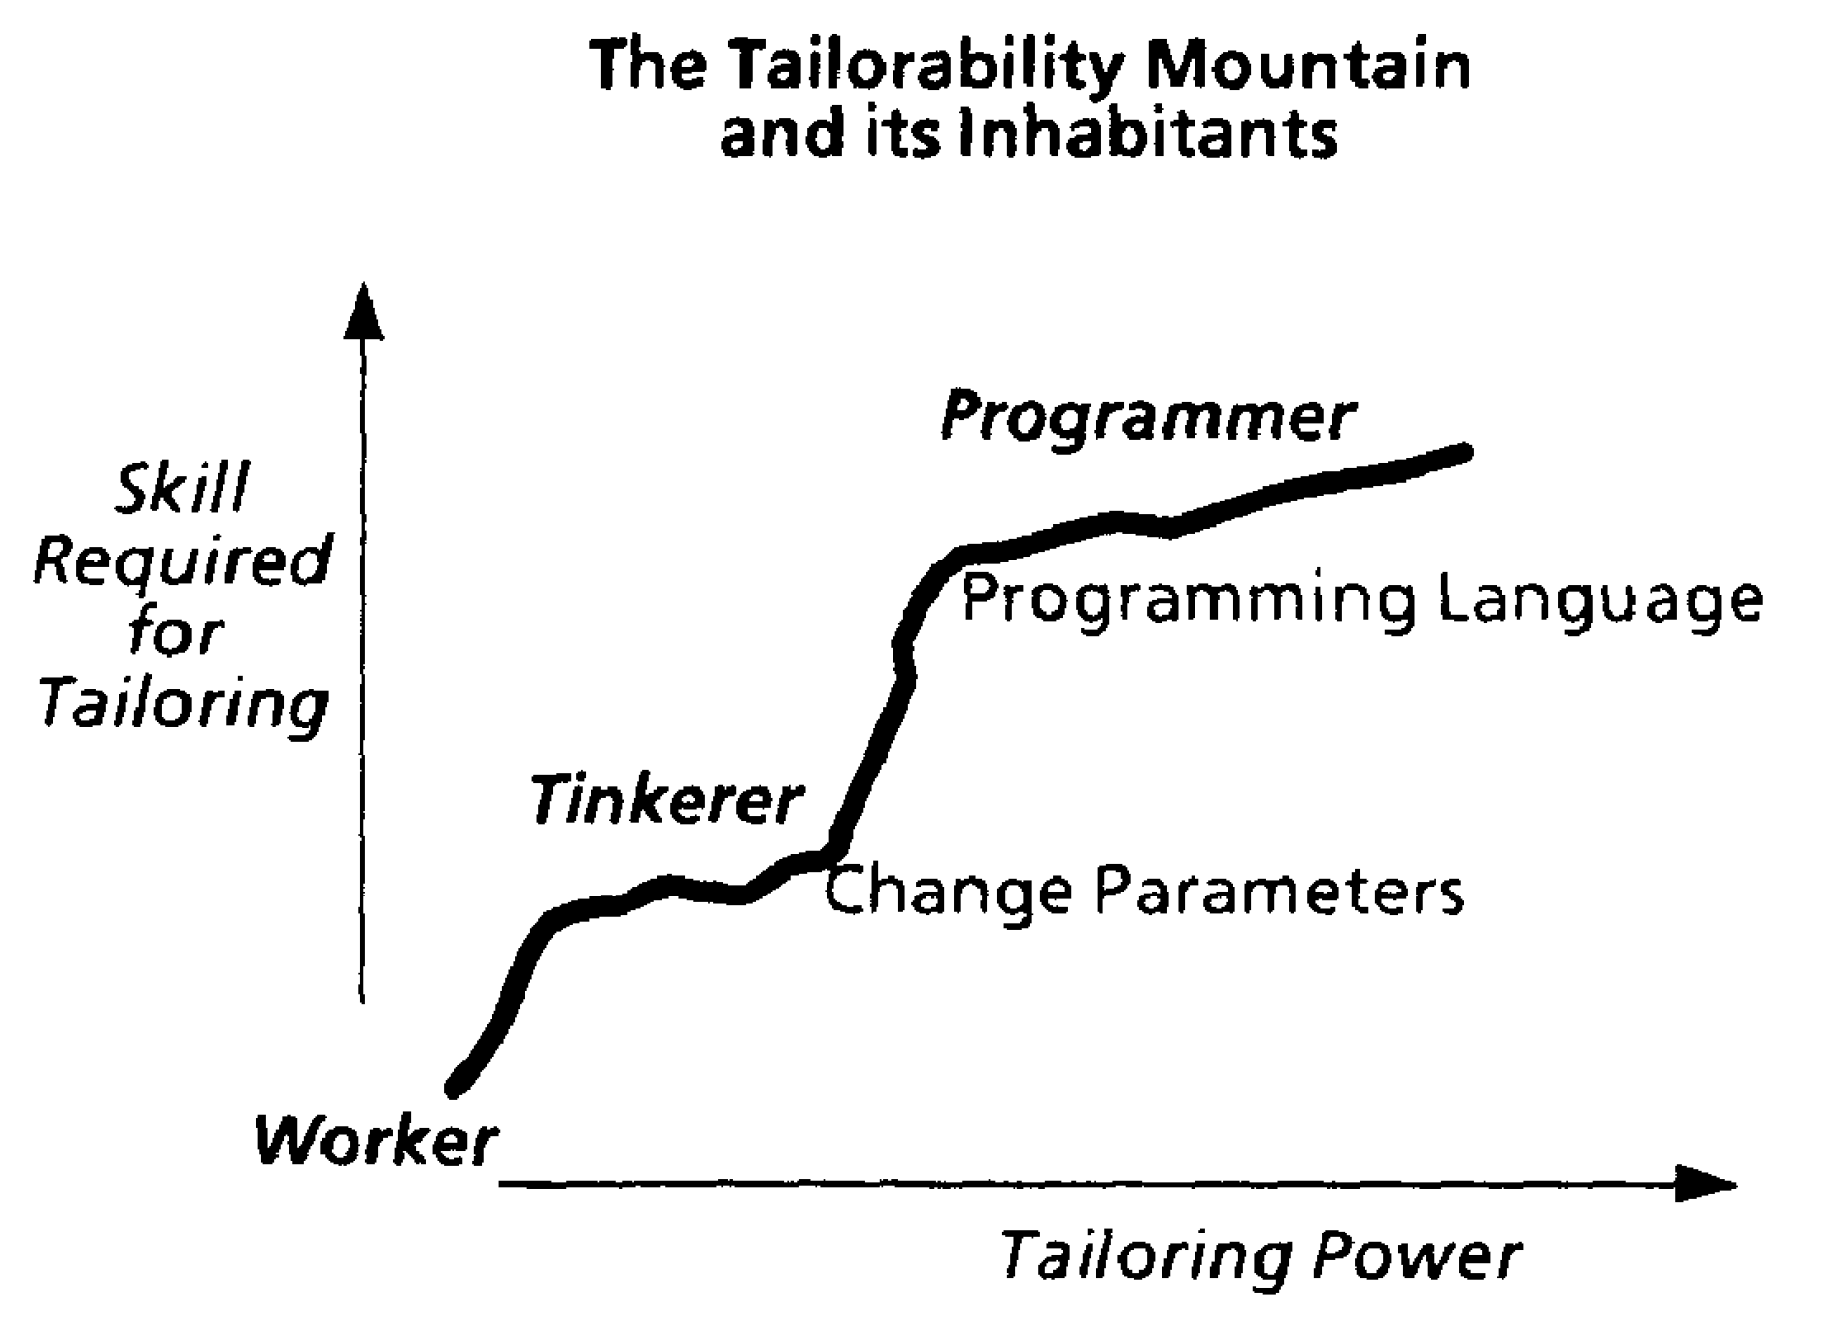
\includegraphics[width=0.6\textwidth]{fig/slope.png}
  \caption{Change in skills required for different kind of system tailoring.
    Some degree of tailoring can be done by learning to change parameters,
    but further tailoring requires mastering a programming language (from \citet{maclean-1990-tailoring})}
  \label{fig:slope}
\end{figure}

~

\subsection{Gradual progression}
A more managerial reason for open software design motivated research on \emph{tailorable systems}
in the 1990s. Because ``it is impossible to design systems which are appropriate for all users and
all situations,'' the researchers ``believe that a useful technique is to have end users tailor
their systems to match their personal work practices.''\endnote{The authors of this quote
\citep{maclean-1990-tailoring} created a system called Buttons that treated the button as
a shareable self-contained unit used for software customization.}
This is illustrated with a diagram (Figure~\ref{fig:slope}), which shows the steep learning
curves necessary to move from user of an application (Worker) to a person who can change
parameters (Tinkerer) and then to a person who can modify the source code (Programmer).\endnote{A similar
diagram appears in a recent discussion of programming substrates and notations by \citet{petricek-2025-limits}.}
An important point, which resonates with a broader discussion about software opacity, is that
supporting tailoring is not merely a technical problem. It also requires ``a culture within which users feel
in control of the system and in which tailoring is the norm.''\endnote{\citet{maclean-1990-tailoring}}

Tailorable systems research focused mainly on office environments and more recent and work in the
area uses the term \emph{malleable software}.
Malleable systems typically aim to allow users to modify software through direct manipulation,
from within the software itself, in a way akin to that used in HyperCard.\endnote{Pioneering
work on direct manipulation has been done by \cite{shneiderman-1983-direct}. \citet{petricek-2025-limits}
explore the limits to which the ``notation for development'' can be the same as the ``notation
for use''.} The approach has been used, among other areas, to enable users to customize
web sites through direct manipulation of tabular data.\endnote{\citet{litt-2020-enduser}}
The argument for malleable software as pluralistic infrastructures ``which reduce the cost of
collaboration between communities''\endnote{\citet{tchernavskij-2019-malleable}} can be made
both on ideological but also on managerial grounds.

\section{Conclusions}
Despite the many visions of open software that can be studied, understood and modified,
most software we use today remains opaque. To understand why, I looked at
two historical case studies. The first followed a debate on information sharing,
while the second followed the development of the web platform. The studies show that
decisions regarding software openness are often based on engineering
or managerial arguments. The virtues of open software systems, such as their understandability
and adaptability, are lost in the quest for more efficient, more scalable, or more
maintainable implementation.

There are pockets of resistance to the growing opacity of software. Some of the visions
discussed earlier continue to be actively developed,\endnote{This includes programming systems
derived from Smalltalk, including Squeak \citep{ingalls-1997-squeak}, which served as the platform
for the development of babylonian programming \citep{rauch-2019-babylonian}, and
Glamorous Toolkit with the vision of moldable development tools \citep{chis-2015-moldable}.}
while new research on malleable software attempts to make software more open and
adaptable. Another perspective on software that has the potential to counter the growing
opacity is the vision of convivial software, inspired by the work of the philosopher Ivan
Illich,\endnote{\citet{illich-1973-conviviality}} that strikes the ``balance between individual
freedom to act and collective freedom from domination''.\endnote{\citet{kell-2020-convivial}}
Stephen Kell identified a number of design heuristics that would lead to a more open,
convivial software systems.\endnote{\citet{kell-2020-convivial}}

A number of decisions that we encountered can be framed as a shift
from shallow embedding (software delegates work to a system within which it
runs) to deep embedding (software reimplements system's functionality).
An interesting question is, what technical or social reasons may prevent such shifts.
I~see two possible answers. First, deep embedding is often more costly to develop.
Many of the developments that we have seen came from large organizations (Google developed
the Google Web Toolkit and used canvas-based rendering for their Google Docs, while
TypeScript has been built by Microsoft).
Smaller software projects are unlikely to have the resources to reimplement
complex logic provided by the system and are thus more likely to use shallow embedding.
Second, deep embedding may be discouraged by certain community culture or a company policy.
As pointed out by Kell,\endnote{\citet{kell-2020-convivial}}
``many of the supposedly technical principles of programming are as much a cultural matter
as a technical one'' and software opacity is no different.

Engineering and managerial decisions currently dominate
the decision making that affects software opacity and, arguably, most other aspects of
software design. If we want software that ``we can control, instead of it controlling
us,''\endnote{Paraphrased from the Free Software bulletin article by \citet{stallman-1986-fsf}.}
we need a conceptual framework for making design decisions about software that does
not favor engineering and managerial decision.



%..\section{Software opacity}
%..\label{sec:opacity}
%..
%..The opacity of software can be seen from a purely technical perspective. As such, it imposes practical
%..limitations that make software inflexible. Ongoing research on tailorable and malleable
%..software attempts to lift such limitations (\S\ref{sec:visions-malleable}). However, from a
%..broader perspective, the opacity of software puts it in an troublesome relationship with society
%..that it increasingly controls.
%..
%..Although this article is mainly concerned with the technical understanding of software
%..opacity, understanding the history of software and the processes that make it more closed
%..in a technical sense contributes to a greater understanding of software in a broader
%..socio-technical sense. For this reason, it is useful to discuss software opacity more
%..generally. I will thus start with a reference to the classic study of \emph{technical objects} by
%..Gilbert Simondon and a more recent literature on software from a philosophical perspective.
%..
%..The role of software in society resembles the role of technical objects, a subject that
%..has been studied in the 1950s by Gilbert Simondon in \emph{On the Mode of Existence of
%..Technical Objects}.\endnote{Published originally in French in 1958 \citep{simondon-2017-existence}.}
%..Simondon's motivation for writing his thesis was the lack of understanding of technical objects in
%..society:\endnote{\citet[p.16]{simondon-2017-existence}}
%..
%..\begin{quote}
%..The most powerful cause of alienation in the
%..contemporary world resides in this misunderstanding of the machine, which is not
%..an alienation caused by the machine, but by the non-knowledge of its nature and
%..its essence, by way of its absence from the world of significations, and its omission
%..from the table of values and concepts that make~up~culture.
%..\end{quote}
%..
%..Today, when software is increasingly ingrained in a wide range of aspects of our lives,
%..and our ``non-knowledge of its nature and its essence'' is ubiquitous,
%..the ``most powerful cause of alienation in the contemporary world'' may well be the
%..misunderstanding of software. The fact that most software is built to hide its inner
%..working is a crucial part of that. As Simondon already pointed out, the ``technical
%..objects that produce the greatest alienation are those meant for ignorant
%..users.''\endnote{\citet[p.255]{simondon-2017-existence}}
%..
%..Simondon called for greater awareness of technical reality and its integration into
%..culture, society and education. A more open software, not meant for ignorant users,
%..may support such aim better than opaque software of the present day.
%..
%..However, we also need to closely examine the software that already exists. This is the
%..approach taken by the field of critical software studies.\endnote{The book edited by
%..\citet{fuller-2008-lexicon} introduces the field. Many interesting accounts have
%..been published as part of the MIT
%..\href{https://mitpress.mit.edu/series/software-studies/}{Software Studies} book series.}
%..Researchers working in the field may closely focus on studying the source code of
%..software,\endnote{An approach known as critical code studies \citep{marino-2020-critical}.}
%..or they may choose to study a specific program from a wide range of perspectives
%..including technical, historical, commercial and cultural.\endnote{The \texttt{10 PRINT}
%..study by \citet{montfort-2012-10print}, which is focused on a single BASIC one-liner,
%..is an excellent example.}
%..
%..A broader critical philosophical examination of software has been written by Federica
%..Frabetti, who focuses on what she describes as the ``main political problem with new
%..technologies'':\endnote{\citet[p.xiii]{frabetti-2014-theory}}
%..
%..\begin{quote}
%..[Technologies] exhibit---in the words of Bernard Stiegler---a `deep opacity'. As Stiegler
%..maintains, `we do not immediately understand what is being played out in technics, nor what
%..is being profoundly transformed therein, even though we unceasingly have to make decisions
%..regarding technics the consequences of which are felt to escape us more and
%..more.'\endnote{\cite{stiegler-1998-technics}}
%..\end{quote}
%..
%..The visions of a more open software, discussed later, imagined a more accessible kind of
%..software that would have the potential to counter such deep opacity. Their failure is thus
%..worth understanding, because the failure of such attempts helps maintain the deep opacity
%..of software technologies.
%..
%..Frabetti tackles the problem in a way that is different from both software studies and from
%..merely technical approaches. ``[R]ather than looking at what people do
%..with software (...) or what software does (...),'' she aims to ``problematize software
%..\emph{as software}, by `undoing' the conceptual system on which it relies for its
%..functioning.''\endnote{\citet[p.xiii]{frabetti-2014-theory} (emphasis original)}
%..Frabetti takes ``historical-cultural and technical narratives,'' including early texts on
%..software engineering and reflections on free software, and uses them ``to problemaitize
%..the intertwining of the technical and the social aspects of software
%..(...).''\endnote{\citet[p.xix]{frabetti-2014-theory}}
%..One of the topics problematized by Frabetti is that of open-source software development
%..methodologies, which she puts in a broader historical software engineering context.
%..I follow the same development from a different perspective (\S\ref{sec:info}), but
%..draw a number of inspirations from Frabetti's work.
%..
%..Frabetti includes technical literature as part of the definition of software, which lets her
%..to transform ``the problem of engaging with software in the problem of reading
%..it.''\endnote{\citet[p.xx]{frabetti-2014-theory}}
%..While I disagree that reading software is sufficient for fully engaging with it,
%..I fully agree with the necessity to tackle the deep opacity of software. Understanding
%..how software becomes opaque in the technical sense, which is the aim of this article,
%..is one of the ingredients of tackling the opacity of software in a broader sense.

